%!TEX root = ../master.tex
\chapter{Building a Tangible Cloud Computing Cluster} 
\label{chap:tangible_cluster}

%!TEX root = ../../master.tex


\begin{theorem}
    Visualization and tangibility are important in conveying cloud computing concepts to accomodate engineering students' learning style preferences. In order to align the students' mental model with the real world, a tangible cloud computing cluster needs to be designed and implemented as a mediating object.
\end{theorem}

\noindent
The previous three chapters introduced many cloud computing concepts. In order to teach and convey these concepts, we introduce a small-scale cloud computing cluster, KubeCloud, as a mediating learning object. The focus of this chapter is the process of specifying, designing, and implementing KubeCloud (Figure~\ref{fig:raspberry_pi_cluster}).

\begin{figure}[H]
    \centering
    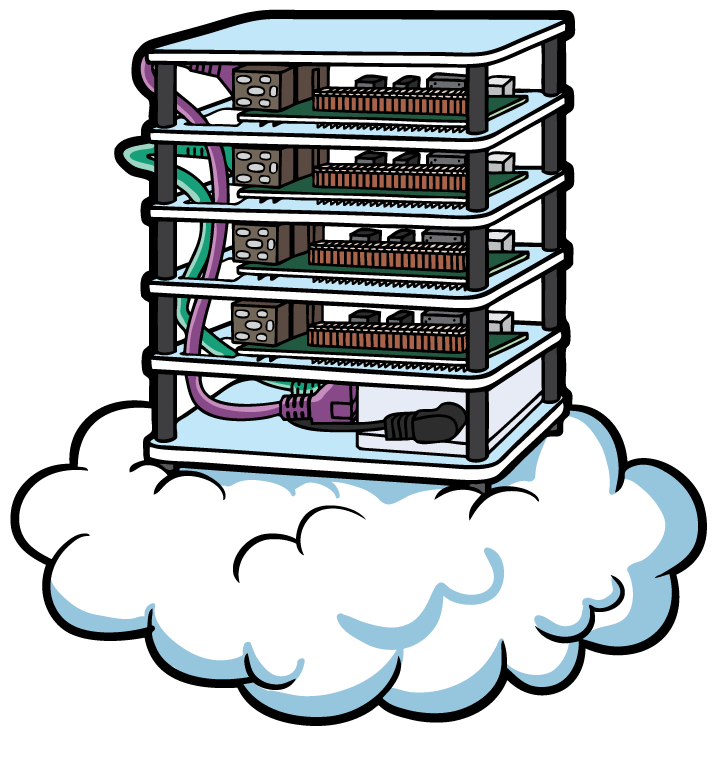
\includegraphics[width=6cm]{figures/raspberry_pi_cluster}
    \caption{Tangible Cloud Computing Cluster}
    \label{fig:raspberry_pi_cluster}
\end{figure}

\noindent
KubeCloud is designed to accommodate the learning style preferences identified by Felder and Silverman (Section~\ref{section:learning_styles}): sensory, visual, active, and sequential. These learning style preferences confirm the need for a learning object. Our experiment, presented later, confirmed three out of four of these preferred learning styles for the students participating in the course presented in this master's thesis. To accommodate the students' preferences and to create an active, sensory learning environment, KubeCloud shall be able to visualize and present concepts and allow for practical hands-on group work to foster social interaction and experimentation. In agreement with Churchill's classification of learning objects, KubeCloud shall be used as a: Presentation object, Practice object, Simulation object, and Conceptual object.
KubeCloud has to be a practice object to foster learning by doing. The workshop format involves the use of KubeCloud as a practice object. Presentations of concepts in cloud computing have to be demonstrated using KubeCloud. KubeCloud will, therefore, act as a presentation object. KubeCloud shall, furthermore, improve the students' skills of real life technologies, and must, therefore, act as a simulation object representing a small-scale real-life system. Lastly, KubeCloud further acts as a conceptual model e.g. by visualizing a small-scale data center.  
%!TEX root = ../../master.tex
\section{Requirements for a Learning Object}
In order to specify the requirements for KubeCloud, we must understand the constraints. The course budget constrained the total cost to DKK 13,000 (USD \$1.957\footnote{DKK-USD currency: 664}). The budget should allow for a minimum of five clusters (20 students with four students per cluster) to be handed out. Another major constraint is the limited implementation time before the course start (thesis start: January 25th, 2016; course start: April 7th, 2016). Before the implementation, a set of requirements are specified for KubeCloud within the limited constraints:

\begin{itemize}
\setlength\itemsep{0.05em}
  \item KubeCloud shall be tangible and allow for practical hands-on experimentation
  \item KubeCloud shall allow for deployment of microservice architecture
  \item KubeCloud shall allow for containerization with Docker
  \item KubeCloud shall allow for container management with Kubernetes
  \item KubeCloud shall allow students to pull out cables to inject failures
  \item KubeCloud shall be able to visualize the state of the cluster
  \item KubeCloud shall visually have characteristics of a server rack
  \item KubeCloud shall be transportable 
  \item KubeCloud shall have a small physical form factor and be able to be carried around in a bag
  \item KubeCloud shall allow for shutdown and restart with a frequency twice a week
  \item KubeCloud shall allow for configuration of the cluster size
\end{itemize}

\noindent
The following sections will describe and discuss the choices made in order to satisfy these requirements.
%%!TEX root = ../../master.tex

%!TEX root = ../../master.tex

\section{Physical Design}
The physical design of KubeCloud is very important in order to satisfy the requirements. The process of building and designing the cluster started out with sketching the possible physical designs. After the initial process of sketching, 3D models of the cluster with the components were made to visualize the cluster and compare it to images of real datacenters. Lastly, an exact 3D model of the individual parts needed to be manufactured was created and sent to the fabricator. The process of the physical design can be seen in Figure~\ref{fig:design_process}.

% SKETCH, 3D, CLUSTER
\begin{figure}[H]%
    \centering
    \subfloat[Sketch]{{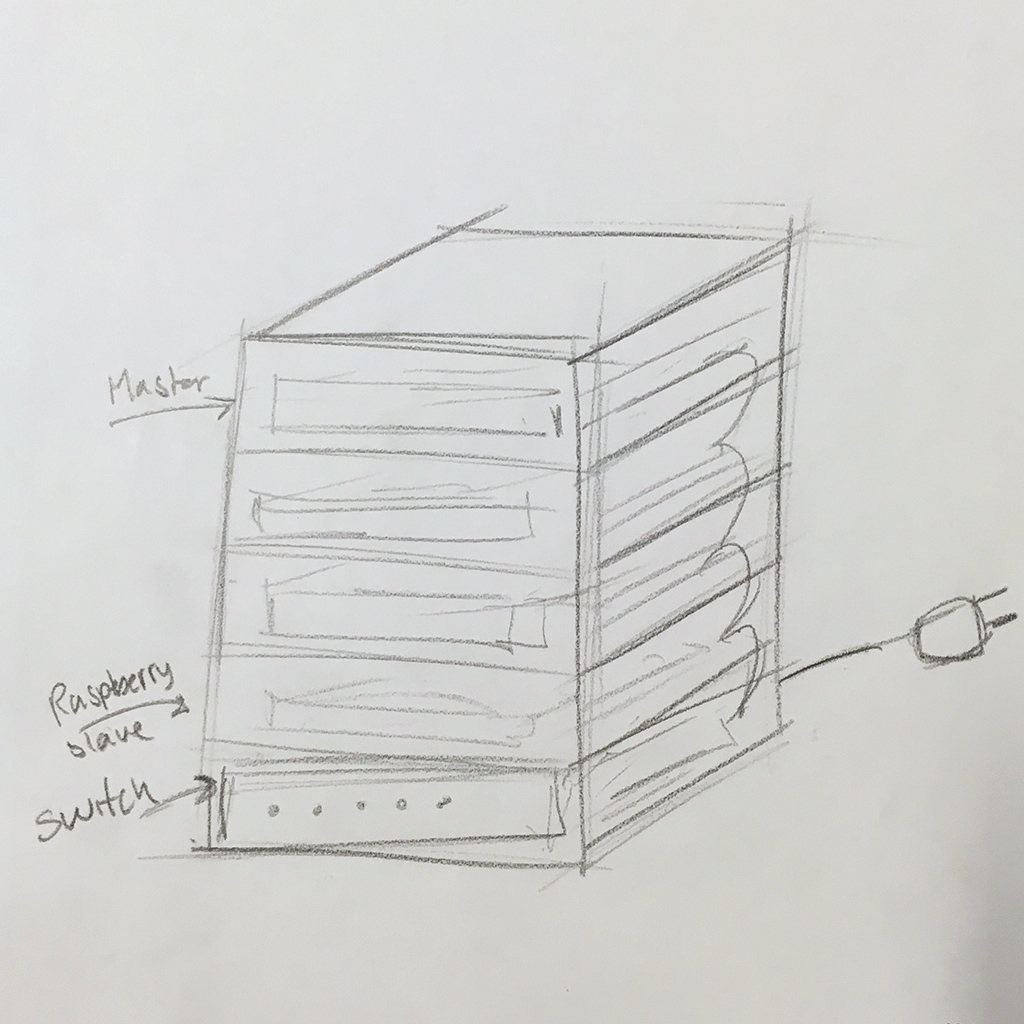
\includegraphics[width=4cm]{figures/cluster/sketch} }}%
    \qquad
    \subfloat[3D model]{{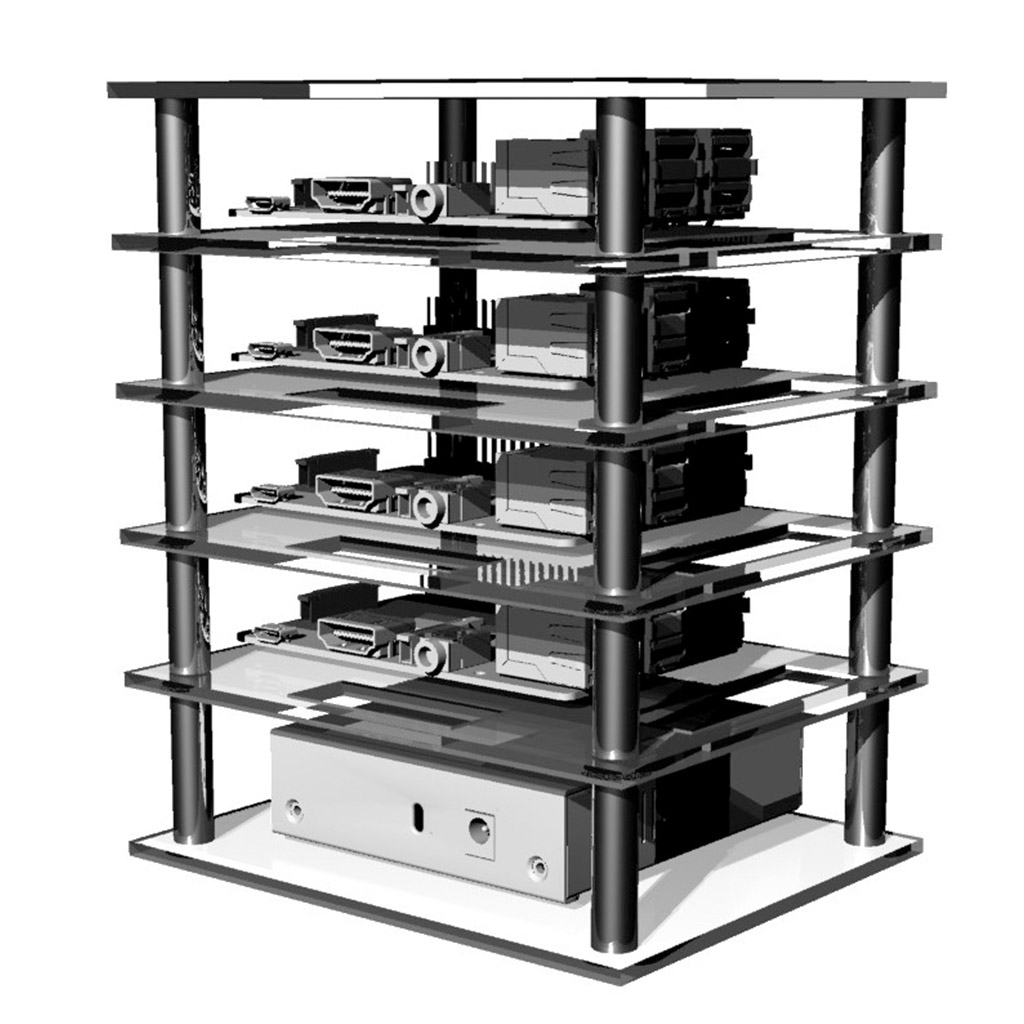
\includegraphics[width=4cm]{figures/cluster/cluster3d_back} }}%
    \qquad
    \subfloat[KubeCloud]{{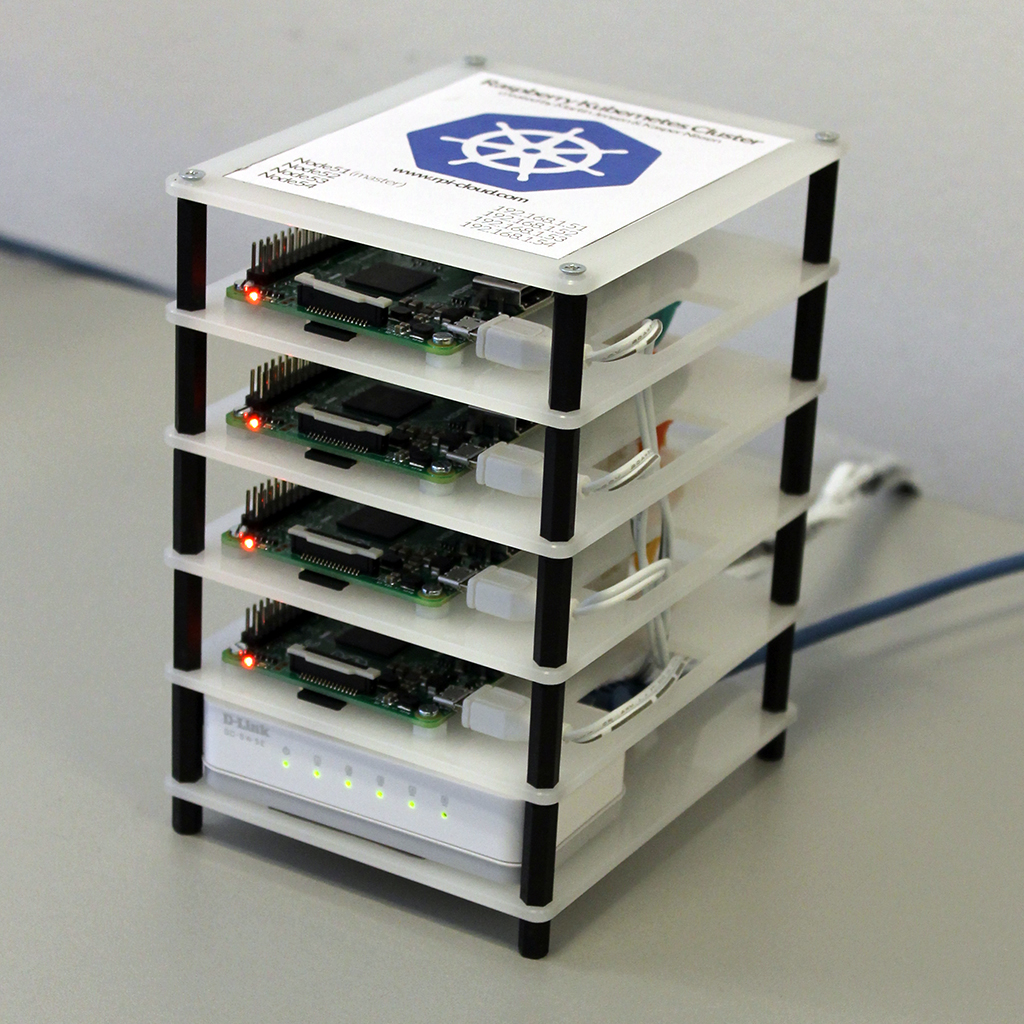
\includegraphics[width=4cm]{figures/cluster/kubecloud_alone} }}%
   
    \caption{Sketch, 3D, and Cluster}%
    \label{fig:design_process}%
\end{figure}

\noindent
The requirement \textit{"KubeCloud shall visually have characteristics of a server rack"} should afford visual associations of working on a scale-model of a data center. KubeCloud consists of stackable layers of Raspberry Pis similar to servers stacked in a server rack in a real data center. Figure~\ref{fig:server_rack} shows the similarity between a server rack and KubeCloud. 

% RACK VS CLUSTER
\begin{figure}[H]%
    \centering
    \subfloat[Rack]{{
\includegraphics[width=4cm]{figures/cluster/rack} }}%
    \qquad
    \subfloat[KubeCloud]{{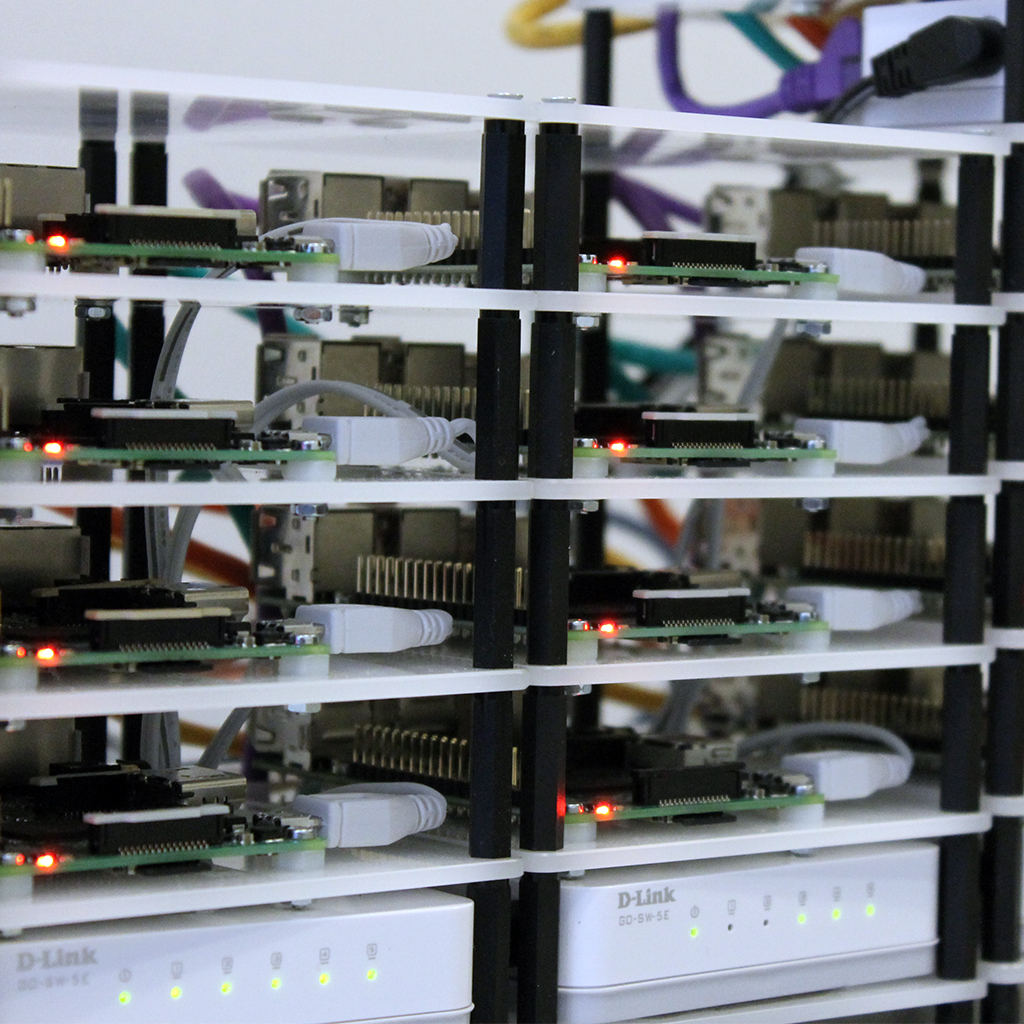
\includegraphics[width=4cm]{figures/cluster/kubecloud_rack} }}%
    \qquad
    \subfloat[KubeCloud]{{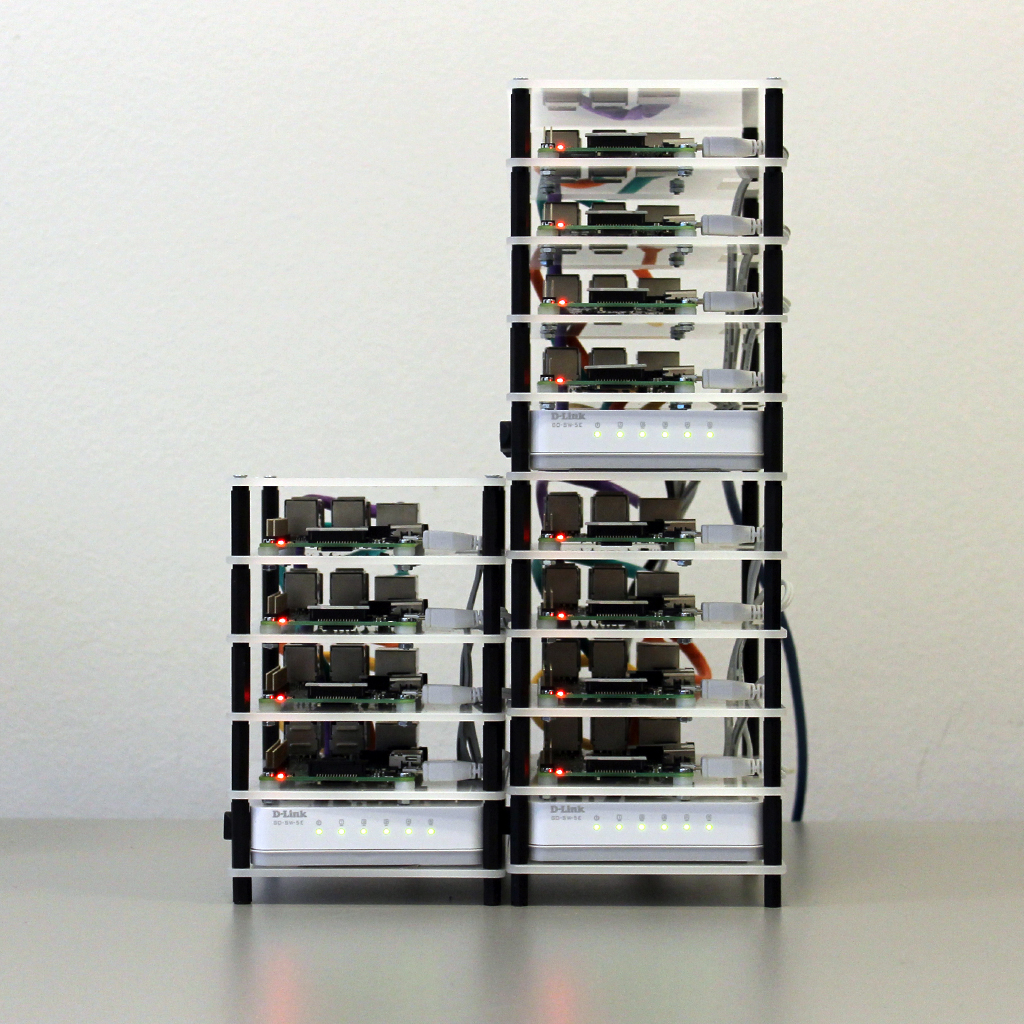
\includegraphics[width=4cm]{figures/cluster/kubecloud_high} }}%
    \caption{Rack Versus Cluster}%
    \label{fig:server_rack}%
\end{figure}

\noindent
Figure~\ref{fig:server_rack} (a) shows a real server rack in a data center. Figure~\ref{fig:server_rack} (b) shows multiple KubeClouds comprising a larger scale data center compared to a single KubeCloud. Figure~\ref{fig:server_rack} (c) shows the dynamism of KubeCloud and the ability to configure the cluster size from a physical perspective. Multiple KubeClouds can easily be mounted together to form a larger small-scale cloud computing environment. This satisfies the requirement of \textit{"KubeCloud shall allow for configuration of the cluster size"}. \\

\noindent
To satisfy the requirement of \textit{"KubeCloud shall have a small physical form factor and be able to be carried around in a bag"}, the power and network connectors are enclosed in the body of the physical design in order to avoid damage during transportation. This further satisfies the requirement \textit{"KubeCloud shall be transportable"}.
The physical size of KubeCloud is made as small as possible within the constraints of the size of the used components (Raspberry Pi and dlinkgo) and the concealment of cables. Figure~\ref{fig:technical_drawings} shows the technical drawings of the two different layers the cluster is comprised of. (a) is the layer the Raspberry Pi is mounted on, (b) is the top and the bottom layer. The 3D model of the two layers can be downloaded from our blog\footnote{\url{http://rpi-cloud.com/guide-how-to-build-a-raspberry-pi-cluster/}}.

% TECHNICAL DRAWINGS
\begin{figure}[H]%
    \centering
    \subfloat[Raspberry Pi layer]{{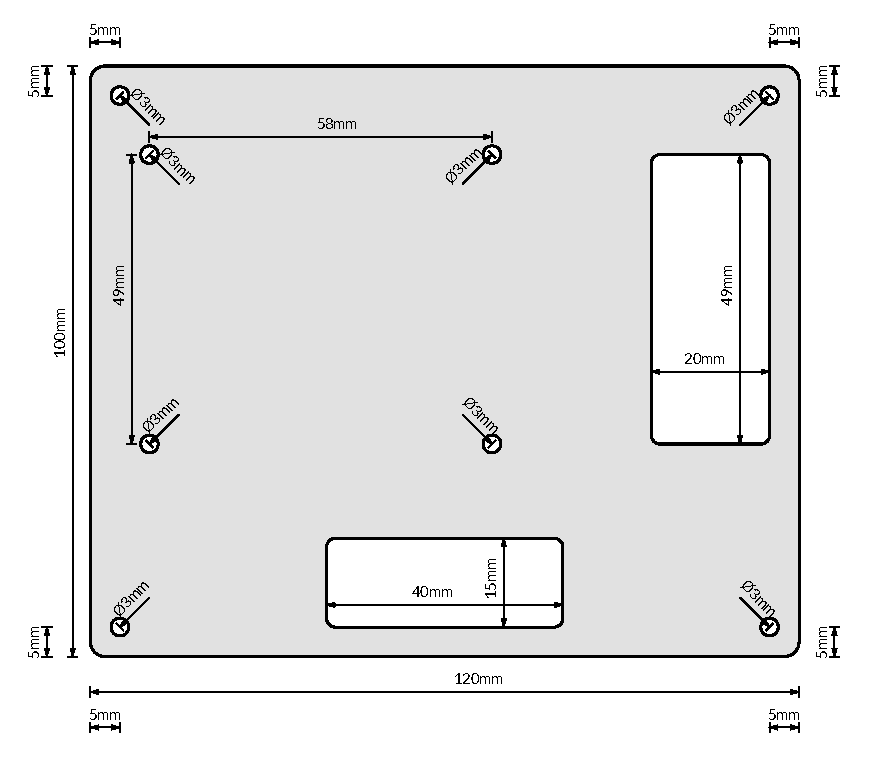
\includegraphics[width=6.5cm]{figures/cluster/raspberry_layer} }}%
    \qquad
    \subfloat[Top bottom layer]{{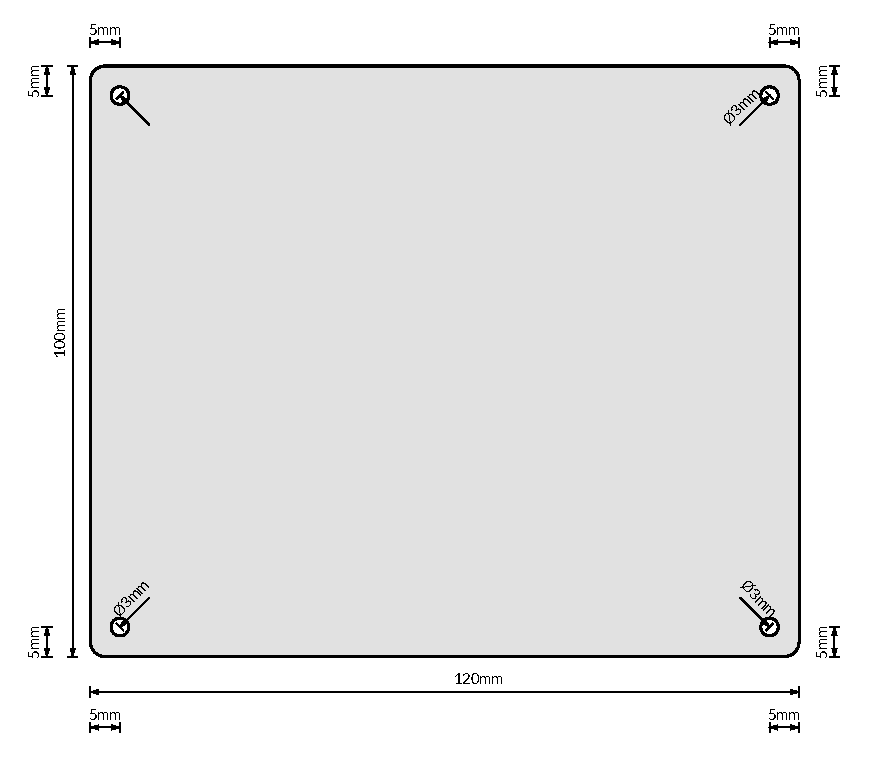
\includegraphics[width=6.5cm]{figures/cluster/top_bottom_layer} }}%
    \caption{Technical Drawings 1:2.5}%
    \label{fig:technical_drawings}%
\end{figure}

\noindent
One of the important purposes of KubeCloud is to demonstrate the effect of failures e.g. network failure. The hole, seen on the right side of Figure~\ref{fig:technical_drawings} (a), makes the ethernet port of the Raspberry Pi accessible and allows for pulling the plug through this hole. This satisfies the requirement of \textit{"KubeCloud shall allow students to pull out cables to inject failures"}.

%!TEX root = ../../master.tex

\section{Hardware}
In order to build KubeCloud, choices of hardware need to be determined within the constraints of the budget. This section will describe the chosen hardware and present the total cost of constructing KubeCloud clusters.  A single KubeCloud will contain four nodes and a switch.

\subsubsection*{Server}

The physical computers (servers) in the cluster have to be chosen. Previous efforts in building small-scale cloud computing environments have chosen the Raspberry Pi as computational units \cite{tso2013glasgow, abrahamsson2013bolzano, cox2014iridis}. The Raspberry Pi is a cheap, yet powerful little machine (900MHz Quad Core Processor, 1GB RAM, ARMv7), that does not require extra cooling, and that easily can be mounted on a surface. Moreover, the Raspberry Pi has the ability to run many different Linux distributions. The low price tag makes it ideal for building a small cluster. Each Raspberry Pi has a 16 GB Kingston Micro SDHC card and is powered by the official Raspberry Pi 2A power supply. 


\subsubsection*{Switch}
The Raspberry Pi's Ethernet port is attached via the USB 2.0 bus, which results in the upstream bandwidth not supporting gigabit speeds. The speed requirements for the switch, therefore, did not play a significant role in the selection.  A 10/100 Mbps switch is sufficient, and the dimensions and the number of ports become the most significant details of the switch. The smaller the better. The chosen switch is a Dlinkgo Fast Ethernet Switch GO-SW-5E with five Ethernet ports (10/100 Mbps). The cables were chosen to be Ethernet Cat5e UTP. The most significant part of choosing cables was length, price, and color of cables. The colors make it easy to distinguish between the nodes in the cluster which is important during exercises.


\subsubsection*{Cost}
The actual cost (excl. VAT) of building a KubeCloud cluster is shown below.

\renewcommand*{\arraystretch}{1}
\begin{longtable}{cp{8cm}rrr}
\toprule
Item   &Description & Price (DKK) & Qty & Total (DKK)\\
\midrule
    \product{Raspberry Pi 2 Model B}{244.15}{4}
    \product{Raspberry Pi 2 power supply}{34.11}{4}
    \product{Kingston MicroSDHC 16 GB}{37.96}{4}
    \product{Dlinkgo Switch GO-SW-5E}{53.16}{1}
    \product{Cat 5e UTP Network cable 0.25m - Orange, Violet, Yellow, Green}{4.00}{4}
    \product{Cat 5e UTP Network cable 1.50m - Blue}{9.60}{1}
\midrule
    &&&& Total \totalttc\\
\bottomrule
\end{longtable}

\noindent
In addition to the KubeCloud clusters, an additional 16-port switch and a router is purchased. The router is needed to create a WiFi network in the classroom for easy access to the clusters. The rack is manufactured at the local tool shop at Aarhus University School of Engineering. To ensure each student gets hands-on time with the cluster, a total of 8 clusters are built. The total cost of the materials used within this present master thesis is: 
\setcounter{cnt}{0}

\begin{longtable}{cp{8cm}rrr}
\toprule
Item   &Description & Price (DKK) & Qty & Total (DKK)\\
\midrule
    \product{Raspberry Pi Kubernetes cluster}{1343.64}{8}
    \product{D-Link DIR-816L AC750 Router}{239.20}{1}
    \product{Sempre Switch 16-port 10/100}{185.00}{1}
    \product{Materials at toolshop (approx)}{200.00}{1}
\midrule
    &&&& Total \totalttc\\
\bottomrule
\end{longtable}

\noindent
The total amount in USD excl. VAT is approximately \$1915\footnote{DKK-USD currency: 664}. The price per student assuming four students per cluster is USD ~\$60. The total cost is within the constrained budget.
%!TEX root = ../../master.tex

\section{Network Topology (Physical)}
The physical network topology of a KubeCloud is set up in a star-topology with the switch as the center of the cluster. Figure~\ref{fig:topology} illustrates this setup.

\begin{figure}[H]
    \centering
    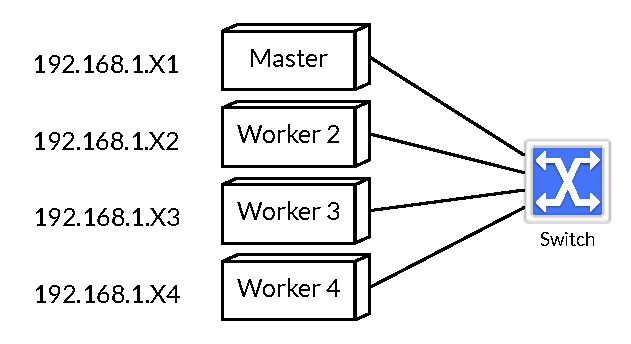
\includegraphics[width=6.5cm]{figures/raspberry_cluster_topology}
    \caption{Network Topology}
    \label{fig:topology}
\end{figure}

\noindent
The static IP convention in each KubeCloud cluster is depicted in Figure~\ref{fig:topology}. The static IP convention assumes clusters of four nodes with the last of the four octets representing a group number and the location of the node in the cluster. The first digit of the last octet determines the group number while the second digit determines the location. The location follows a convention of the master node being the topmost physical location. The following worker nodes and IPs are increasing downwards, e.g. group 1 will have the following nodes: 192.168.1.11 (Master), 192.168.1.12 (Worker 2), 192.168.1.13 (Worker 3), 192.168.1.14 (Worker 4). \\

\noindent
An alternative to static IPs is to use zero-configuration networking implementation such as Avahi. A test was conducted in the beginning of the project, but the stability of using Avahi was not satisfying in our case. Therefore, the static IP convention was chosen instead. Static IPs are rigid and can limit the number of nodes in a cluster following the naming convention, but stability was the crucial parameter. This way of configuring the IPs of the cluster allows for easily connecting the single cluster to the entire network of clusters used in the classroom. This decoupling of clusters allows for custom configuration of cluster sizes, which will be explained in the software section of this chapter. When putting it all together, the clusters are again set up in star-topology as depicted in Figure~\ref{fig:topology_overall}.

\begin{figure}[H]
    \centering
    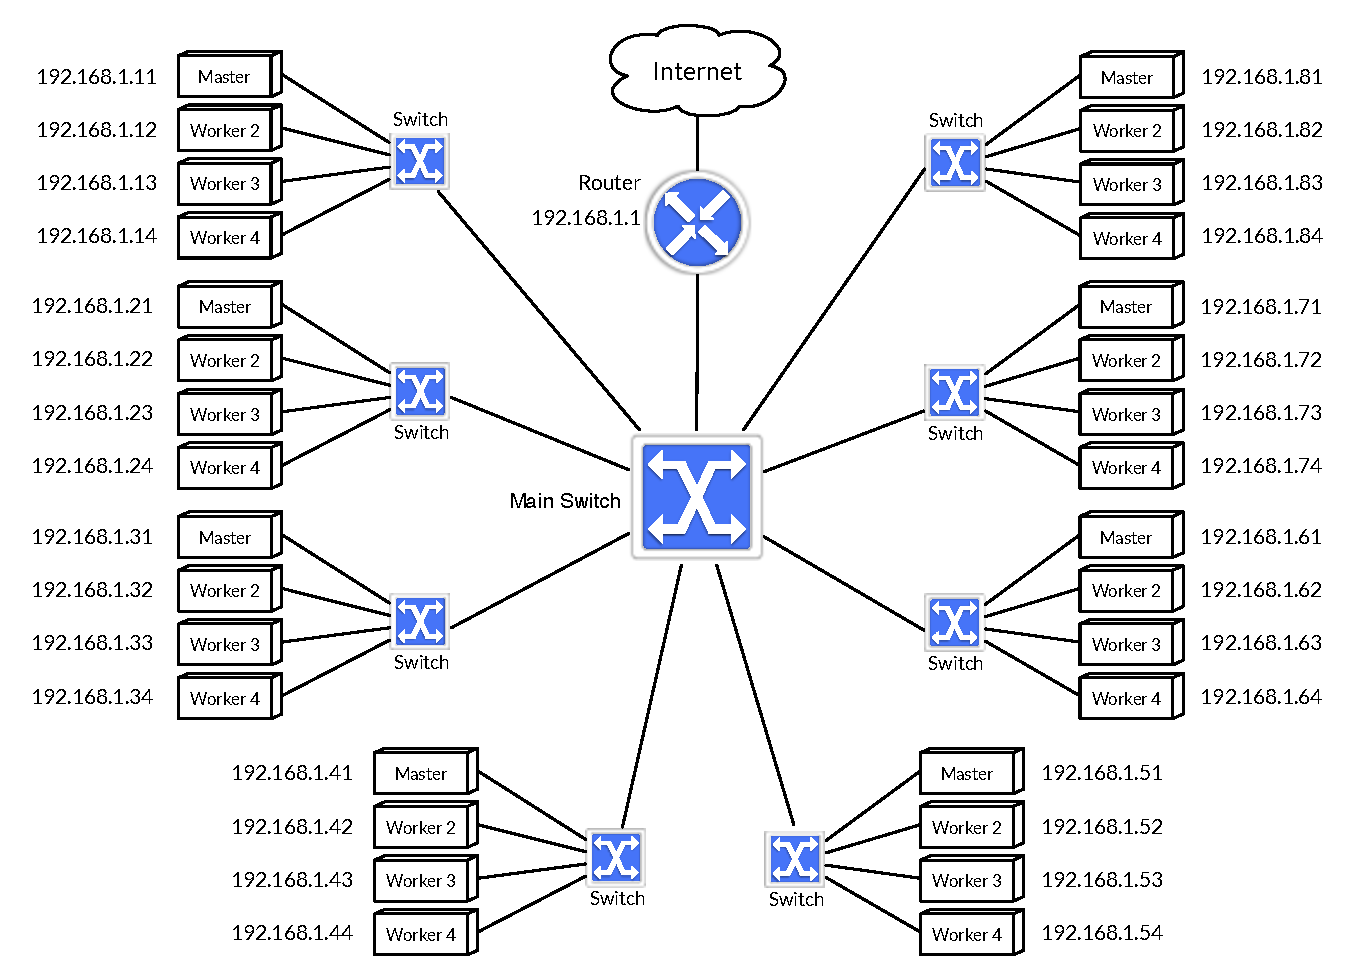
\includegraphics[width=\textwidth]{figures/overall_topology}
    \caption{Overall Network Topology}
    \label{fig:topology_overall}
\end{figure}

\noindent 
The router act as the gateway for the internet connection needed to access the Docker Hub repositories. 
%!TEX root = ../../master.tex
\section{Software}
The previous sections described the process of designing and building a physical cluster. We now turn the focus to the decisions made regarding software in building KubeCloud. The involved layers will be described and discussed from the operating system layer to the application layer.


\subsection*{Operating System}
Hypervisors are often used in data centers (Chapter~\ref{chap:fundamentals_cloud}) and could be an interesting topic to investigate. The limited resources on a Raspberry Pi, however, does not allow for powerful enough partitions of the resources into virtual machines. Furthermore, the partitioning contradicts the purpose of the physical representation of the concepts in cloud computing. KubeCloud is, therefore, a bare-metal cluster without virtual machines. \\

\noindent
The choice of operating system (OS) is important since the rest of the software need to run on top of it. Stability is one of the most important properties of the OS for KubeCloud.
A Linux distribution is needed to run Docker and Kubernetes. We did not have a particular distribution preference but looking at the available options in the ARM community led to the choices of HypriotOS, Raspbian, or Arch Linux. The intention was to build on top of already configured distributions to keep the focus on the usage of the cluster.

\subsubsection*{The Road to a Stable OS}
Several different configurations of operating systems combined with different Docker and Kubernetes versions have been tried out on the road to stability to address the requirement \textit{"KubeCloud shall allow for shutdown and restart with a frequency twice a week"}. \\

\noindent
\textit{HypriotOS with k8s-on-rpi} \\
At first, HypriotOS\footnote{\url{http://blog.hypriot.com/downloads/}}(v0.6.1) was tried out. HypriotOS is an extension of the default Raspberry Pi OS (Raspbian).  Installation of HypriotOS is easy, and it has Docker installed out of the box. HypriotOS seemed like a good solution since Kubernetes was easy to get up and running on the clusters using k8s-on-rpi\footnote{\url{https://github.com/awassink/k8s-on-rpi}}. Unfortunately, stability issues arose after restarting the clusters, which became evident when Kubernetes became unresponsive. The time used for scheduling of pods experienced an increase and failed in many cases. \\


\noindent
\textit{HypriotOS with kubernetes-on-arm} \\
Another Kubernetes project called kubernetes-on-arm\footnote{\url{https://github.com/luxas/kubernetes-on-arm}} was installed on top of HypriotOS (v0.6.1), but the stability issues were still present. The debugging was time-consuming since we had to flash SD cards, assign static IPs, install Kubernetes, and wait for the errors to appear. \\


\noindent
\textit{ArchLinux with kubernetes-on-arm} \\
Since the common factor in the two previous configurations was the operating system, a new operating system was investigated. An ArchLinux installation from the kubernetes-on-arm project turned out to (almost) be the end of the road of our stability issues. In order to automate and adjust the project to our setup, scripts were created for automation purposes. These scripts are described in further detail in the upcoming section on Kubernetes. \\


%% Docker
\subsection*{Docker}
As described in Section~\ref{sec:role_of_os_and_hypervisors}, containers such as Docker have gained much attention the last couple of years because of the benefits they provide. Figure~\ref{fig:flow_spring_software} shows Docker's role in the cluster. Applications (Spring Boot) are containerized into a Docker image with the needed dependencies. The Kubernetes infrastructure is using the Docker images to manage the cluster.
\begin{figure}[H]
    \centering
    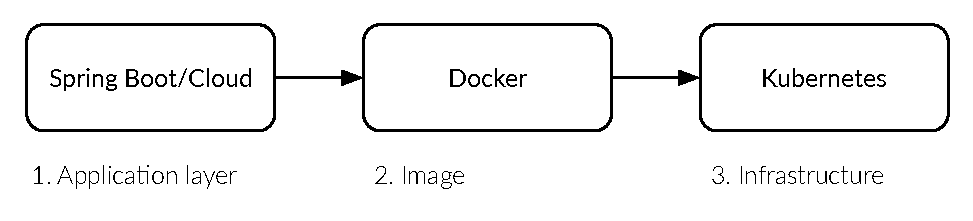
\includegraphics[width=12cm]{figures/flow_overview}
    \caption{Flow Overview}
    \label{fig:flow_spring_software}
\end{figure}

\noindent
Installing Docker on a Raspberry Pi is not difficult, but since the Raspberry Pi runs on ARM architecture, all Docker images must be built for ARM. Most developer machines do not use ARM, and cross-compilation or building on an ARM device is, therefore, necessary. One of the ideas behind Docker is that applications and dependencies can be packaged together and recreated in the production environment. The ARM architecture limitation is unfortunate, but it has not been a big problem. Two very similar base images of Java 8 have been used for the ARM and amd64 architectures to accommodate this challenge.

\noindent The previously described ArchLinux configuration comes with the installation of Docker used in KubeCloud.
%% /Docker

\subsection*{Kubernetes}
Kubernetes (v1.2) was chosen as cluster management system for several reasons. The previously mentioned transformation from being machine-oriented to application-oriented combined with the increased tendency of containerization led to the decision of using containers and Kubernetes. Furthermore, containers are more lightweight than virtual machines, and since the Raspberry Pi has restricted resources compared to a server it seemed like a good idea to reduce the overhead. In order to illustrate concepts of resilience, Kubernetes offers several interesting approaches to adaptive capacity (Figure~\ref{fig:our_resilience_definition}) on the infrastructure level resilience. Among those are replication, heartbeats, and automatic rescheduling when pods fail, which leads to rapidity. Many of Kubernetes' concepts can be used to illustrate resilience on a physical cluster. \\

\noindent
Kubernetes is used to manage Docker containers on the Raspberry Pis in KubeCloud. Each Raspberry Pi node is registered as a node in the cluster and is thereby a small-scale bare-metal server running Kubernetes. On managed solutions such as Google Container Engine, a virtual machine is used per node instead of a Raspberry Pi. In KubeCloud, Kubernetes schedules workloads (containers) across the different Raspberry Pis (nodes). \\

\noindent
As previously described, the road to stability led to a configuration with ArchLinux and the kubernetes-on-arm project. Kubernetes-on-arm furthermore comes with many features such as a command-line tool to enable masters and workers and to manage add-ons. One of the most important add-ons has been the KubeDNS add-on, which makes it possible to use a service's name as the hostname instead of using IP addresses. The command-line tool makes it possible to change the role of any of the nodes seen in Figure~\ref{fig:topology_overall}. A master can with a single command be configured as a worker of another master. In our setup, each cluster has a master and three workers, but this structure can easily be changed if a cluster with e.g. seven workers is needed.
The command-line tool has furthermore served as a building block in the previously mentioned automation scripts. Scripts for startup and shutdown of the clusters were created to ease the startup process and, more importantly, to make sure that the cluster was shut down correctly. The shutdown script disables Kubernetes on all nodes, waits for them to finish, and shuts down the Raspberry Pis. \\


\noindent One of the essential assumptions in Kubernetes is that pods can communicate with other pods regardless of which host they are scheduled on. As described in Section~\ref{sec:cluster_management}, all pods have their own IP address, which frees the user of Kubernetes, in most cases, for port mappings between container ports and host ports. In order to fulfill this assumption, Kubernetes can use different implementations depending on the platform it is deployed to. KubeCloud leverages an open source project called flannel which is included in kubernetes-on-arm. \\

\noindent
Flannel is a software defined overlay network, also called a virtual network, that assigns a subnet to each host for use with the container runtime, which in this case is the Docker engine. An example of the virtual network provided by flannel is shown in Figure~\ref{fig:flannel}.

\begin{figure}[H]
    \centering
    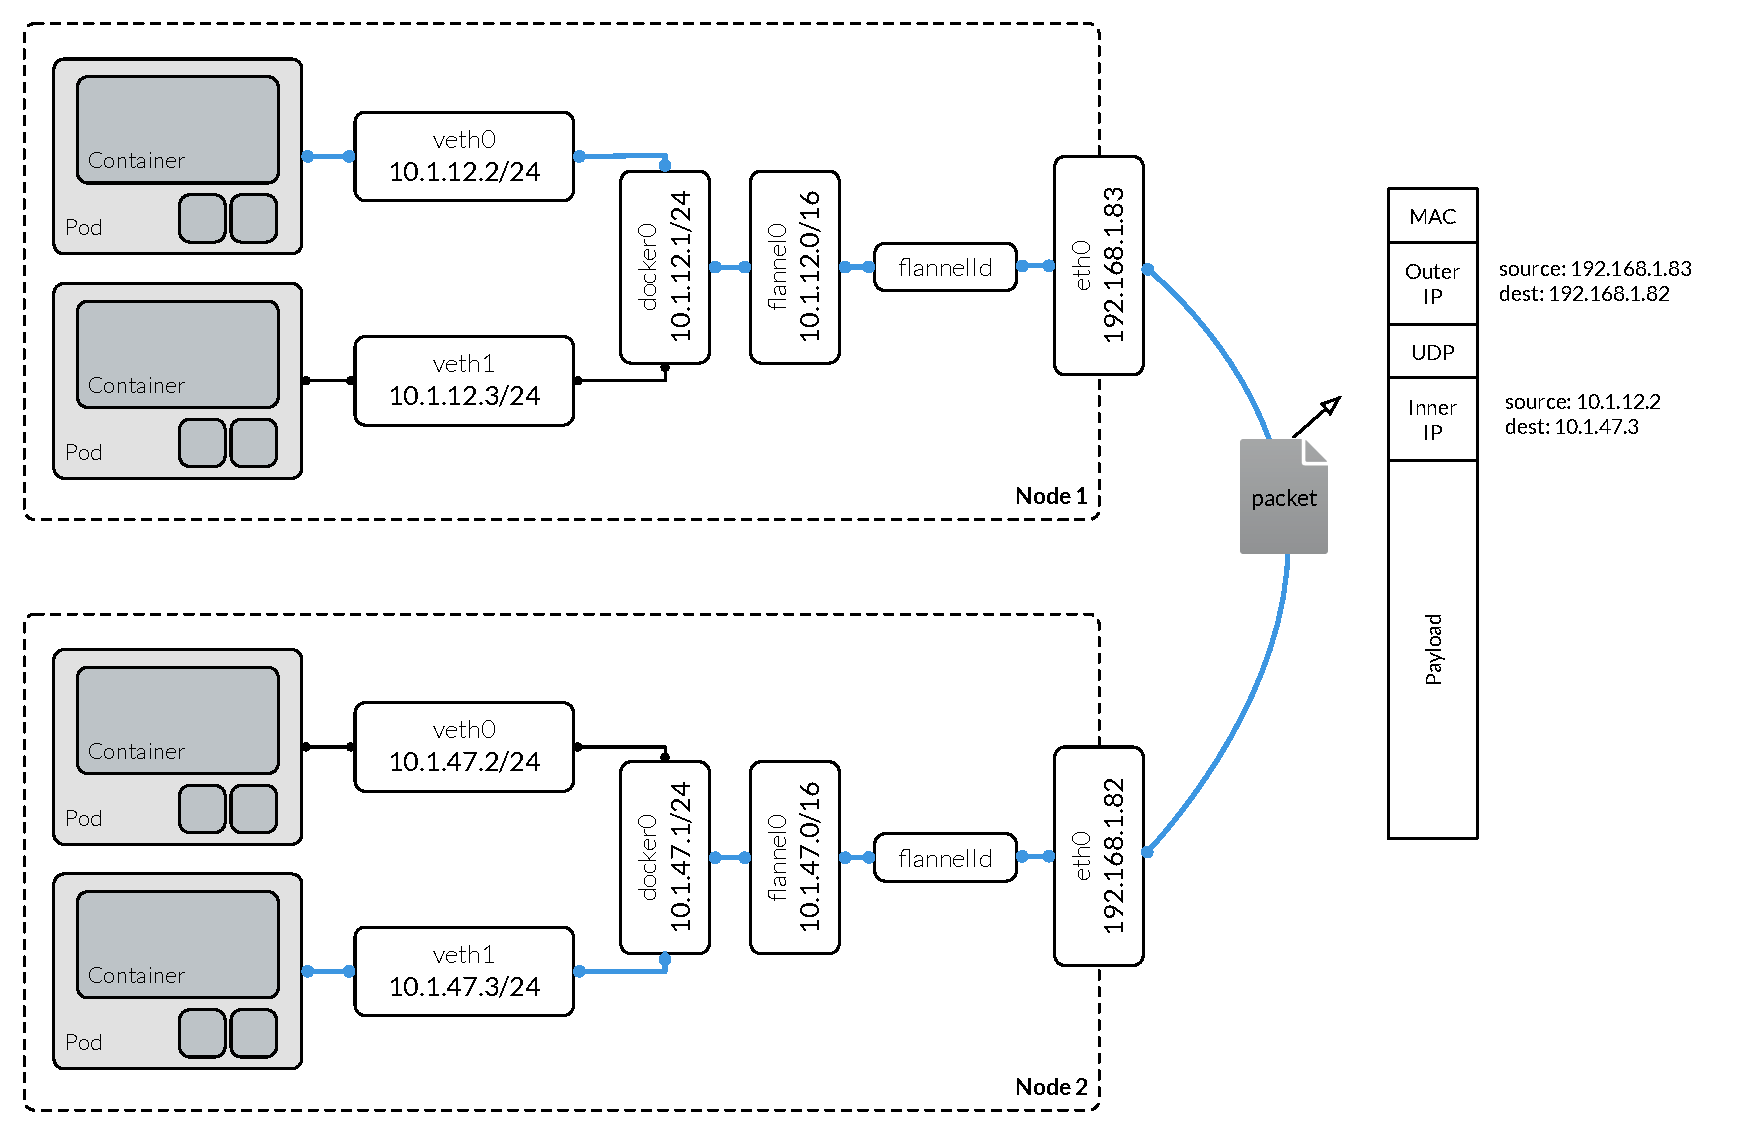
\includegraphics[width=\textwidth]{figures/kubernetes/flannel_networking}
    \caption{Flannel Networking}
    \label{fig:flannel}
\end{figure}

\noindent Figure~\ref{fig:flannel} shows two nodes in a Kubernetes cluster. Each node has the Docker engine and a flannel agent running. The example shows how the pod-to-pod communication is achieved. Every pod is assigned a virtual IP provided by the docker0 subnet. The docker0 subnet is controlled and assigned by flannel. Flannel stores these configurations in etcd, which makes it possible to map between host IP and virtual IP. As seen from the payload, Node 1's packet contains an inner IP destination with the virtual IP of the pod and an outer IP destination with the host machine's IP (Node 2). This mapping helps decouple pod and machine, and multiple pods on the same machine can expose the same port.
%!TEX root = ../../master.tex

\subsection*{Visualizer}
Visualization is expected to play an important role in students' learning and the bridging between cloud computing and the physical machines, especially since engineering students tend to be visual learners. This fulfils the requirement \textit{"KubeCloud shall be able to visualize the state of the cluster"}. KubeCloud allows for injecting failures e.g. by pulling the network cables (Figure~\ref{fig:visualizer_node_failure}). However, it can be hard to understand and grasp what is going on in Kubernetes. Hence, a visualization tool is needed. 

\begin{figure}[H]%
    \centering
    \subfloat[Node failure]{{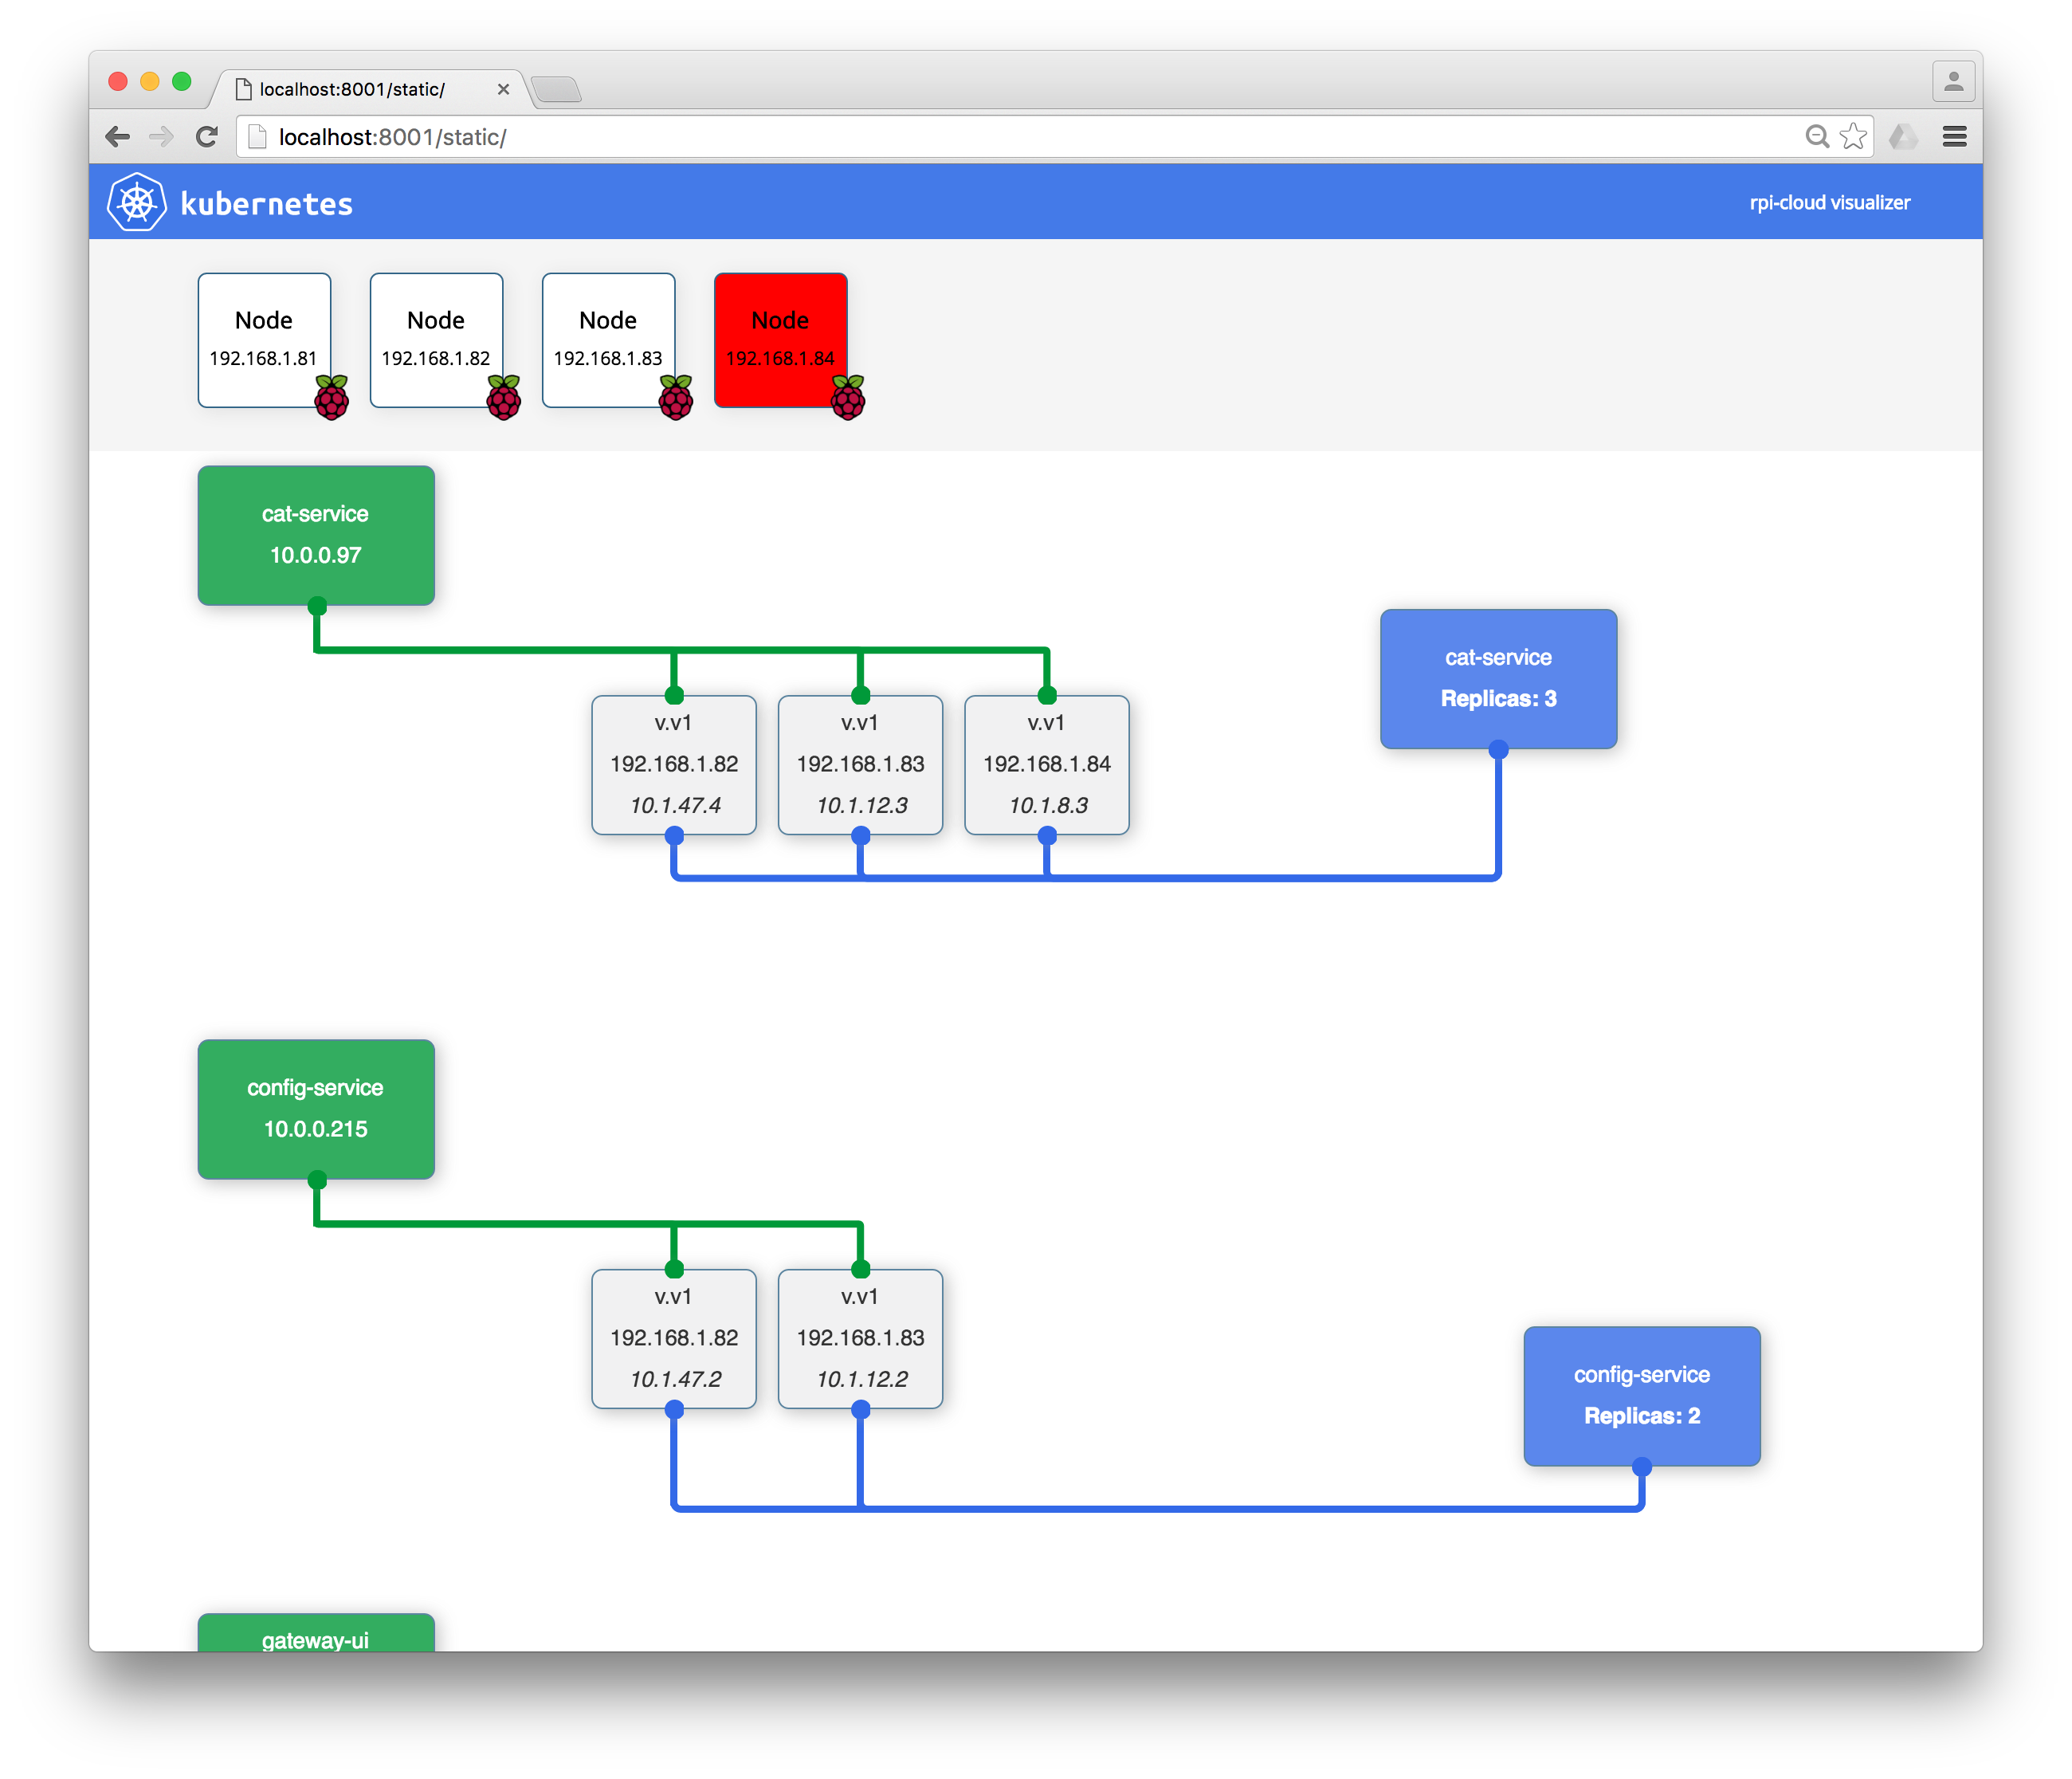
\includegraphics[width=7cm]{figures/visualizer/node_fail} }}%
      \qquad
    \subfloat[Rescheduling]{{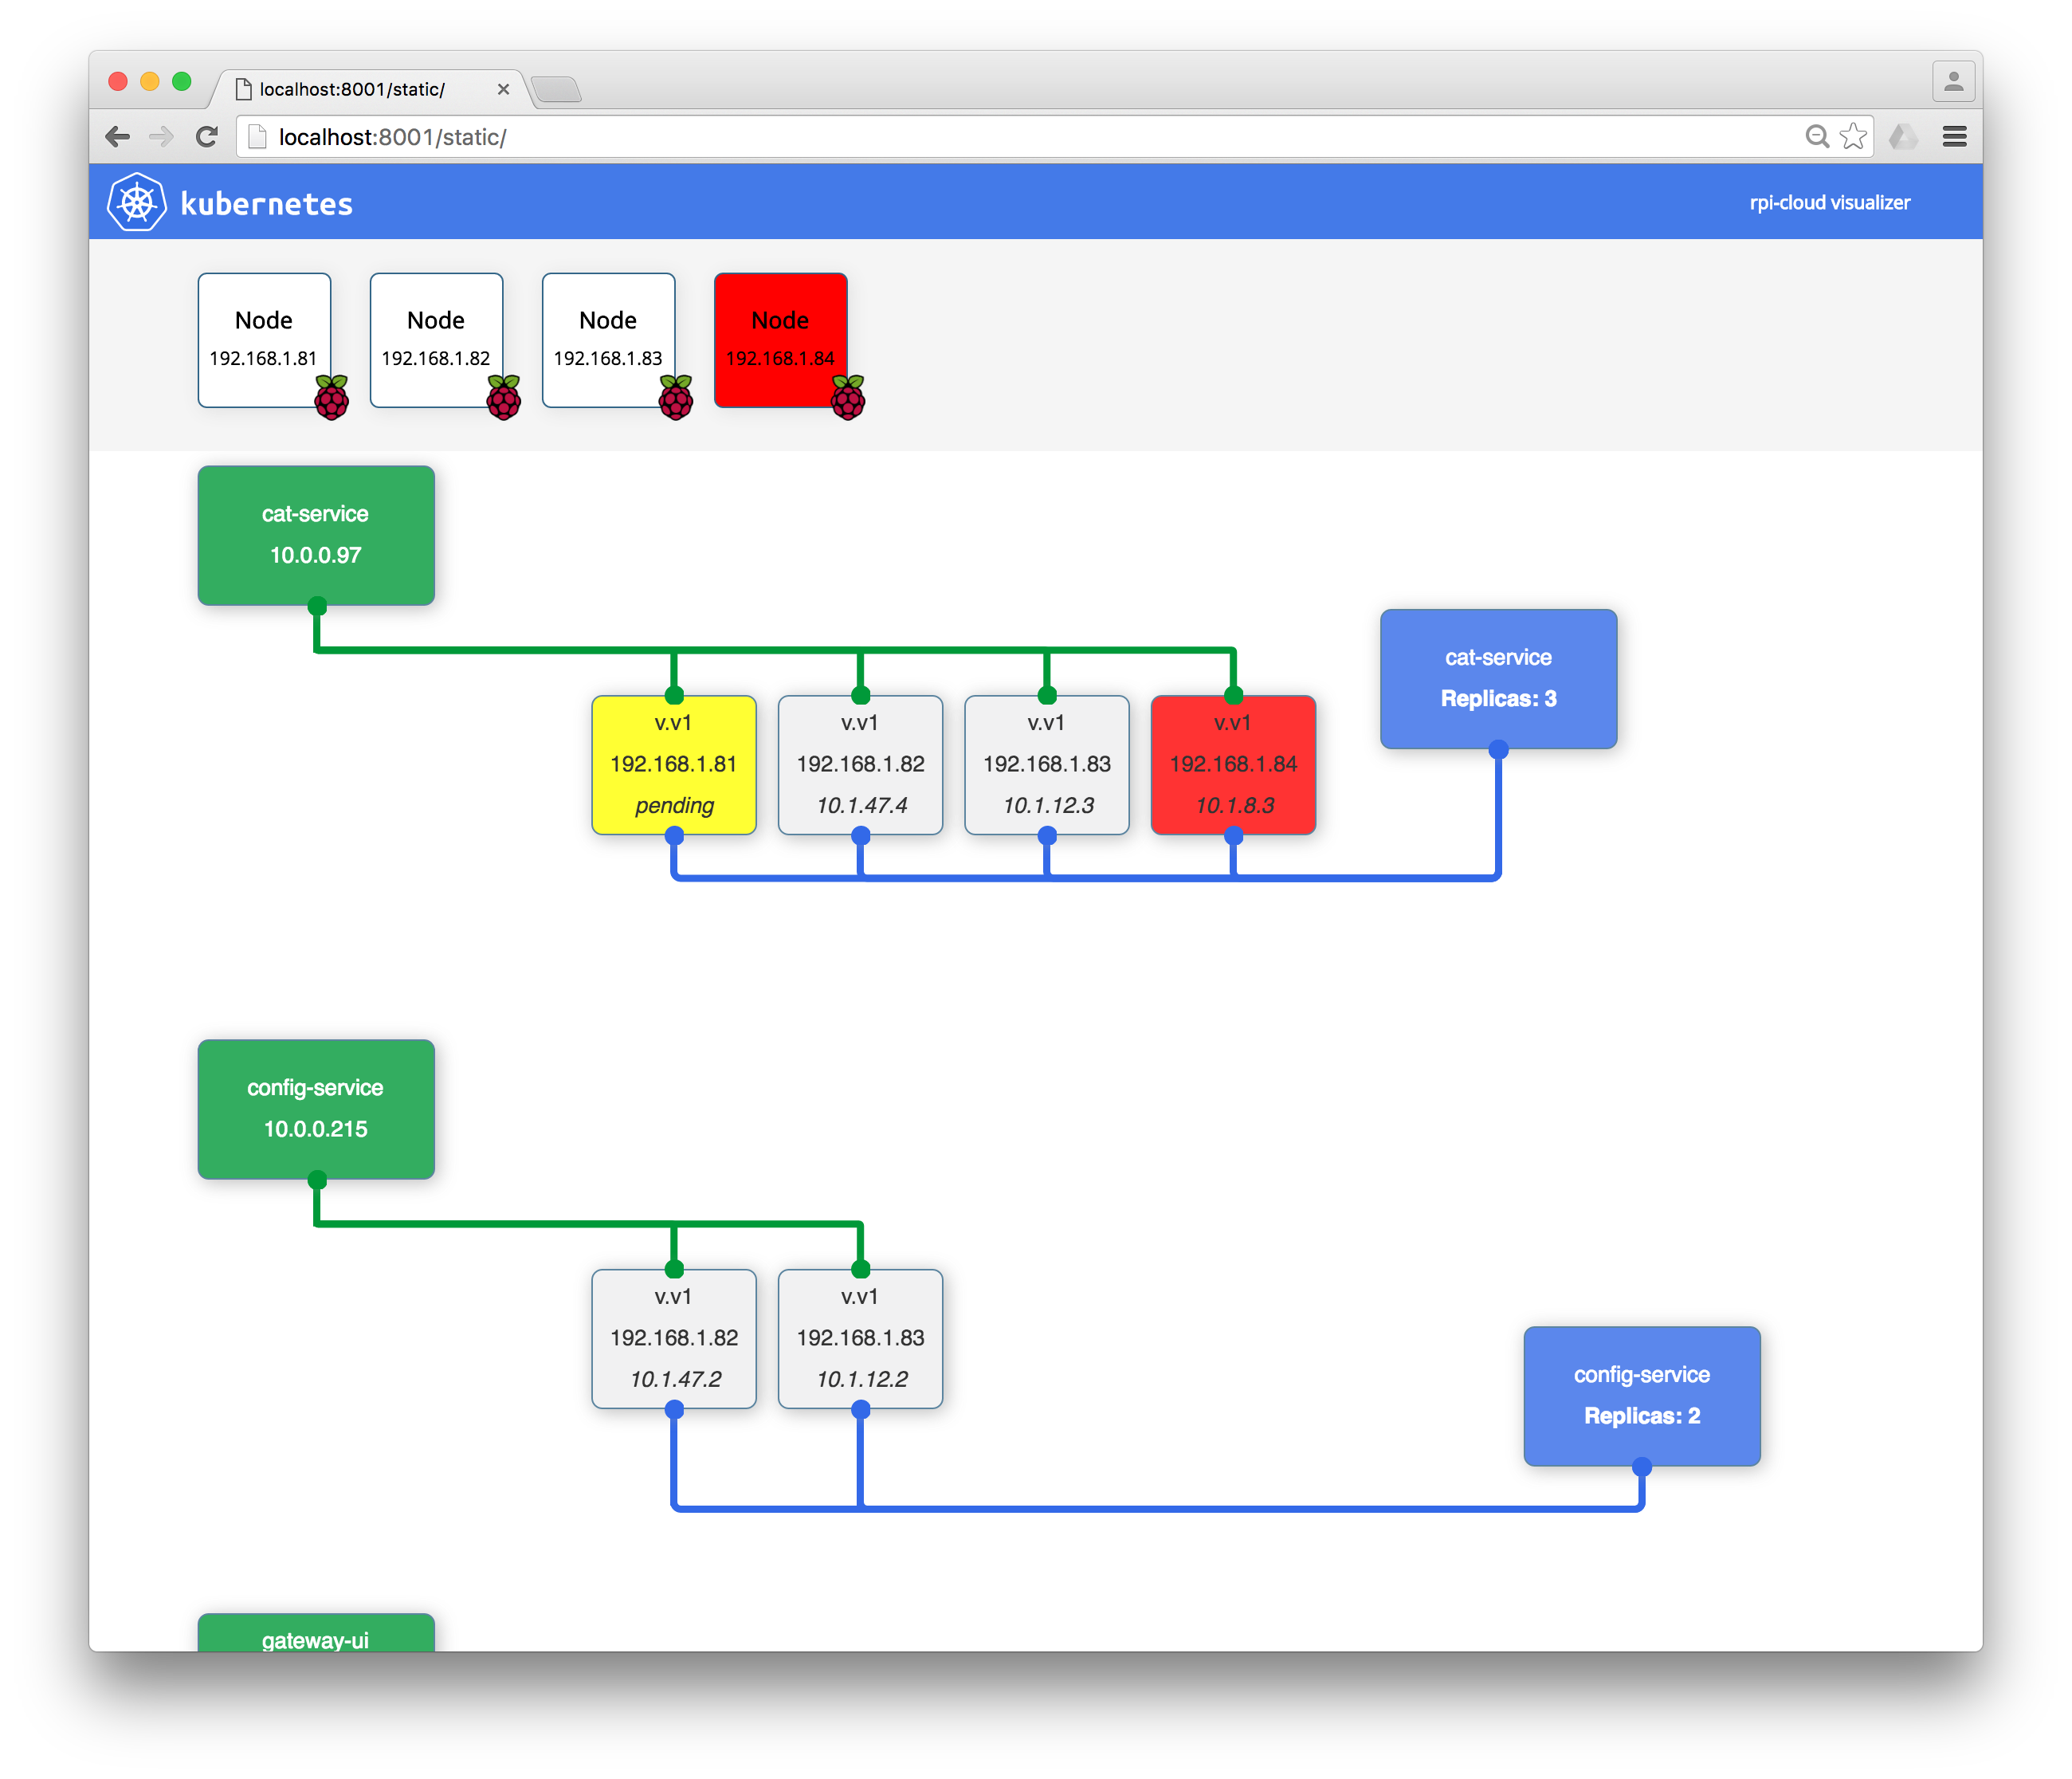
\includegraphics[width=7cm]{figures/visualizer/node_fail_reschedule} }}%
          \qquad
    \subfloat[Recovered]{{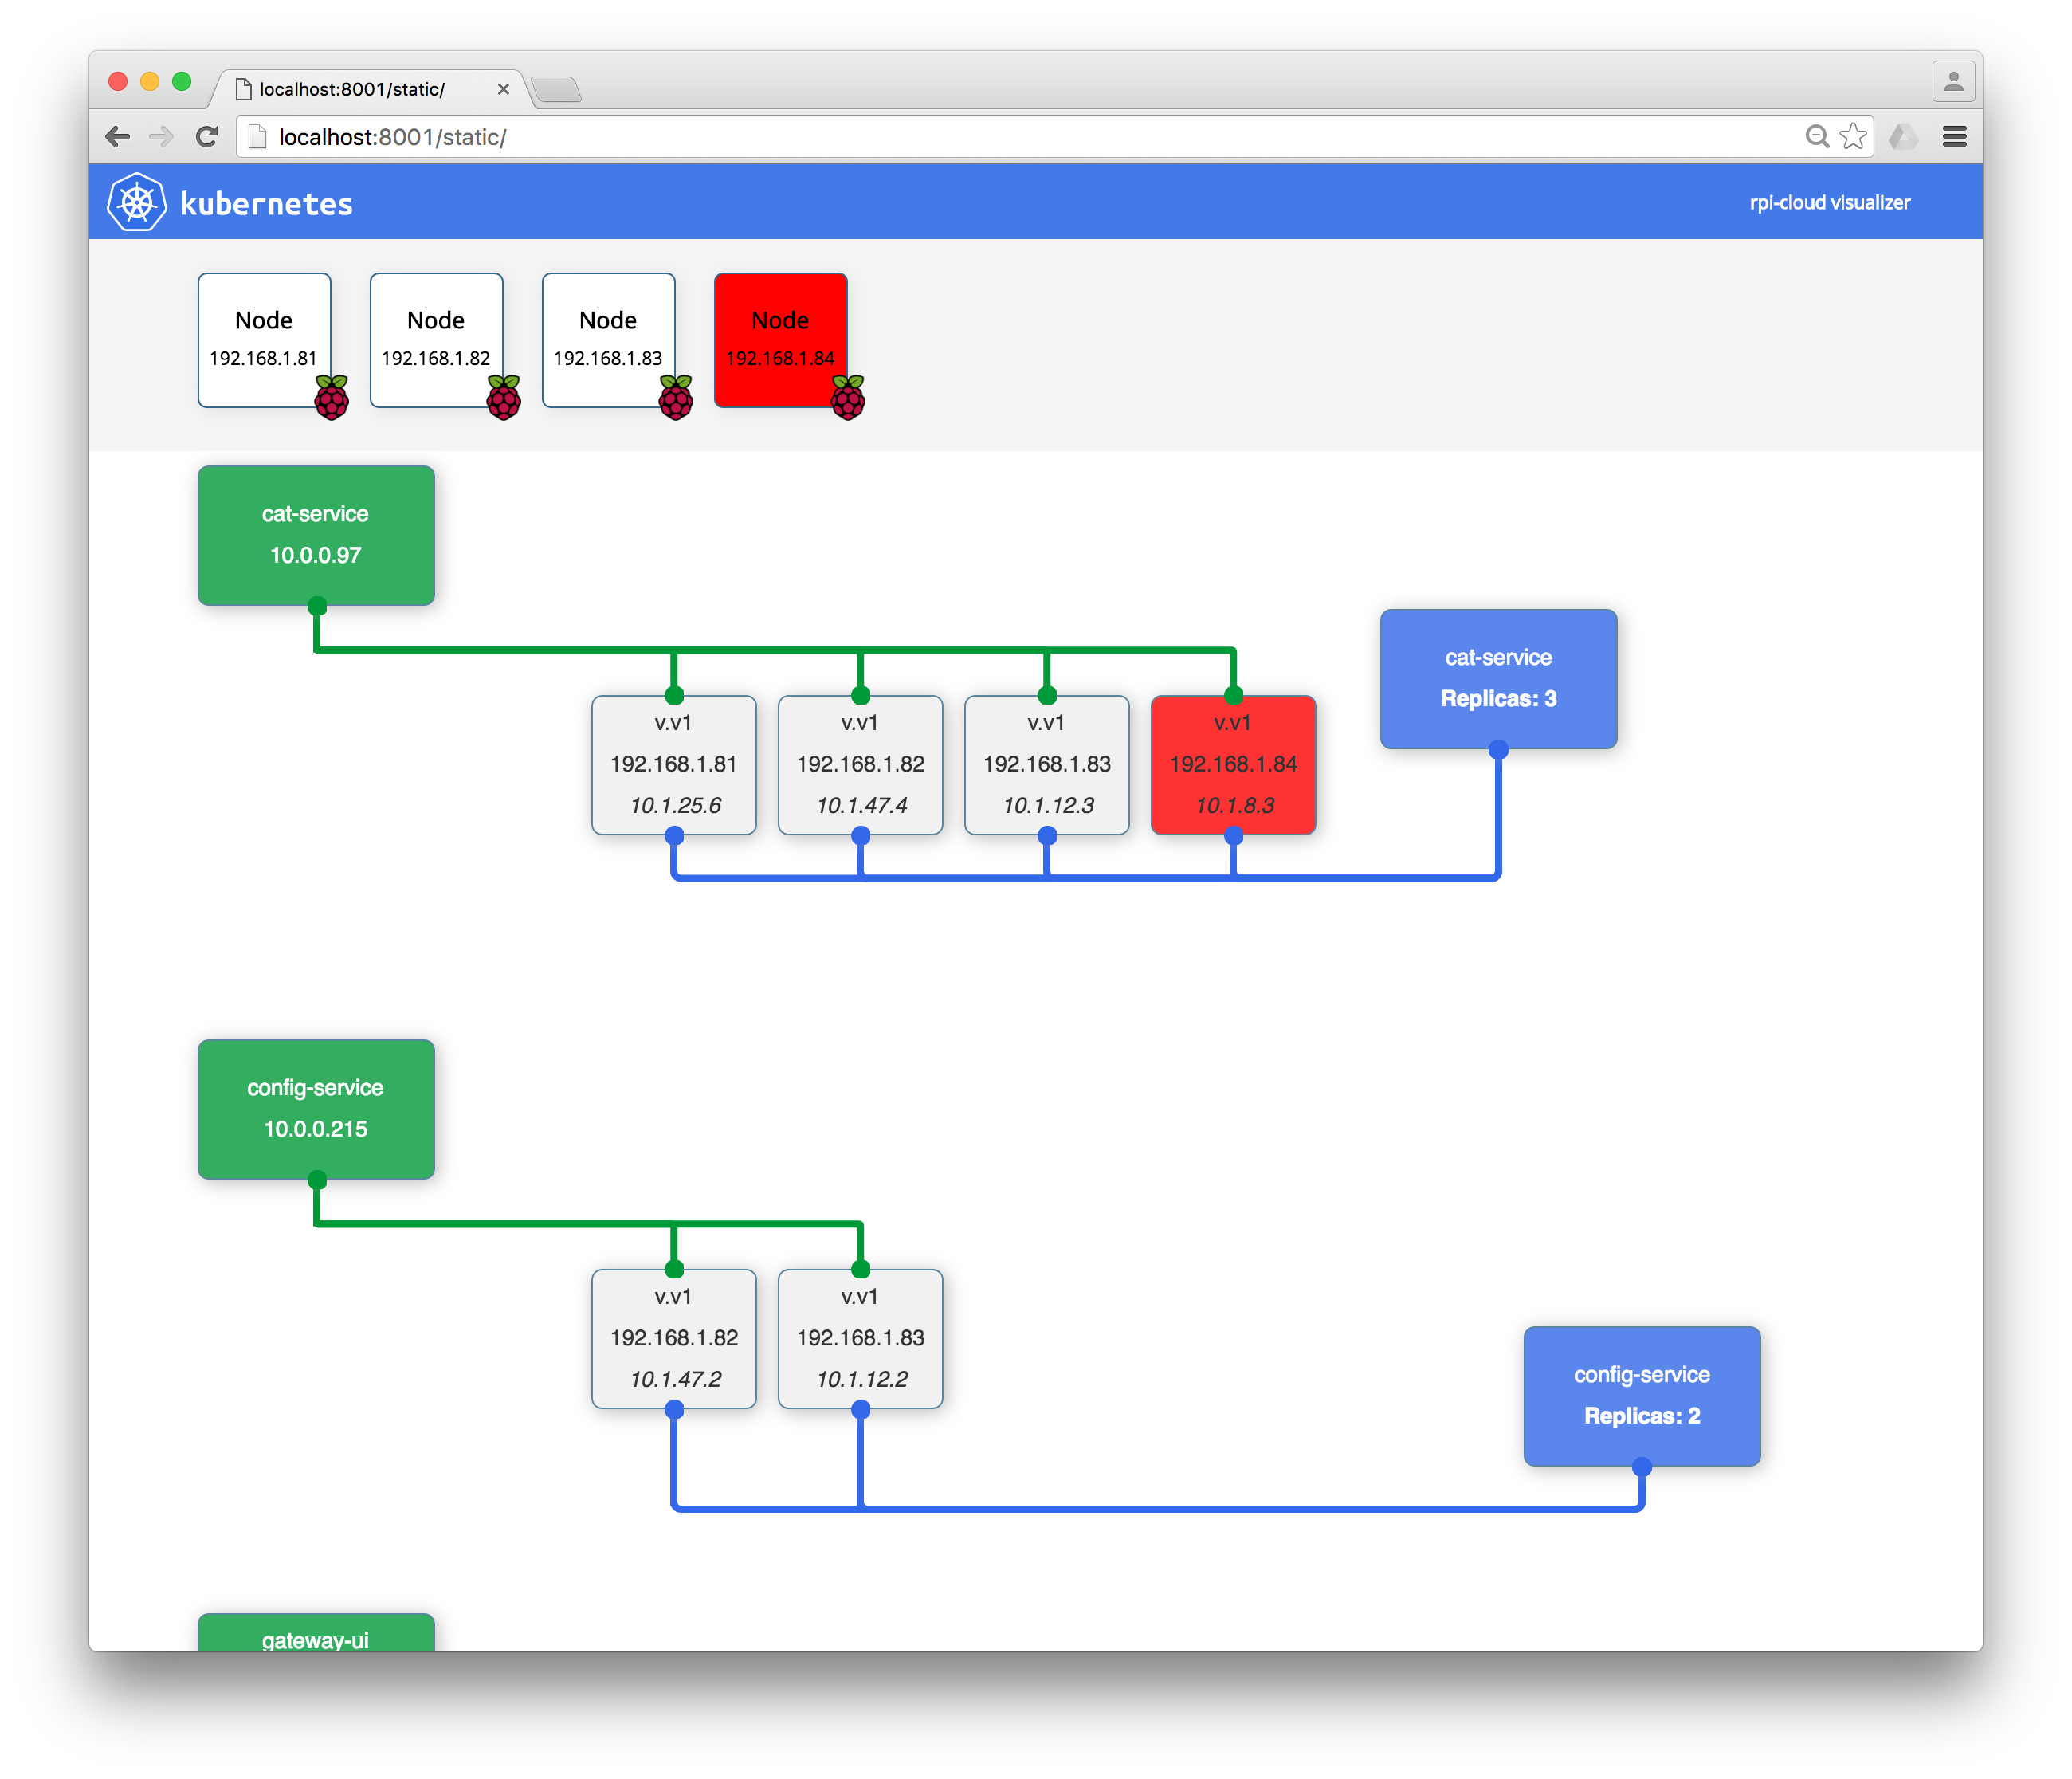
\includegraphics[width=7cm]{figures/visualizer/node_fail_clean_up} }}%
          \qquad
    \subfloat[Clean up]{{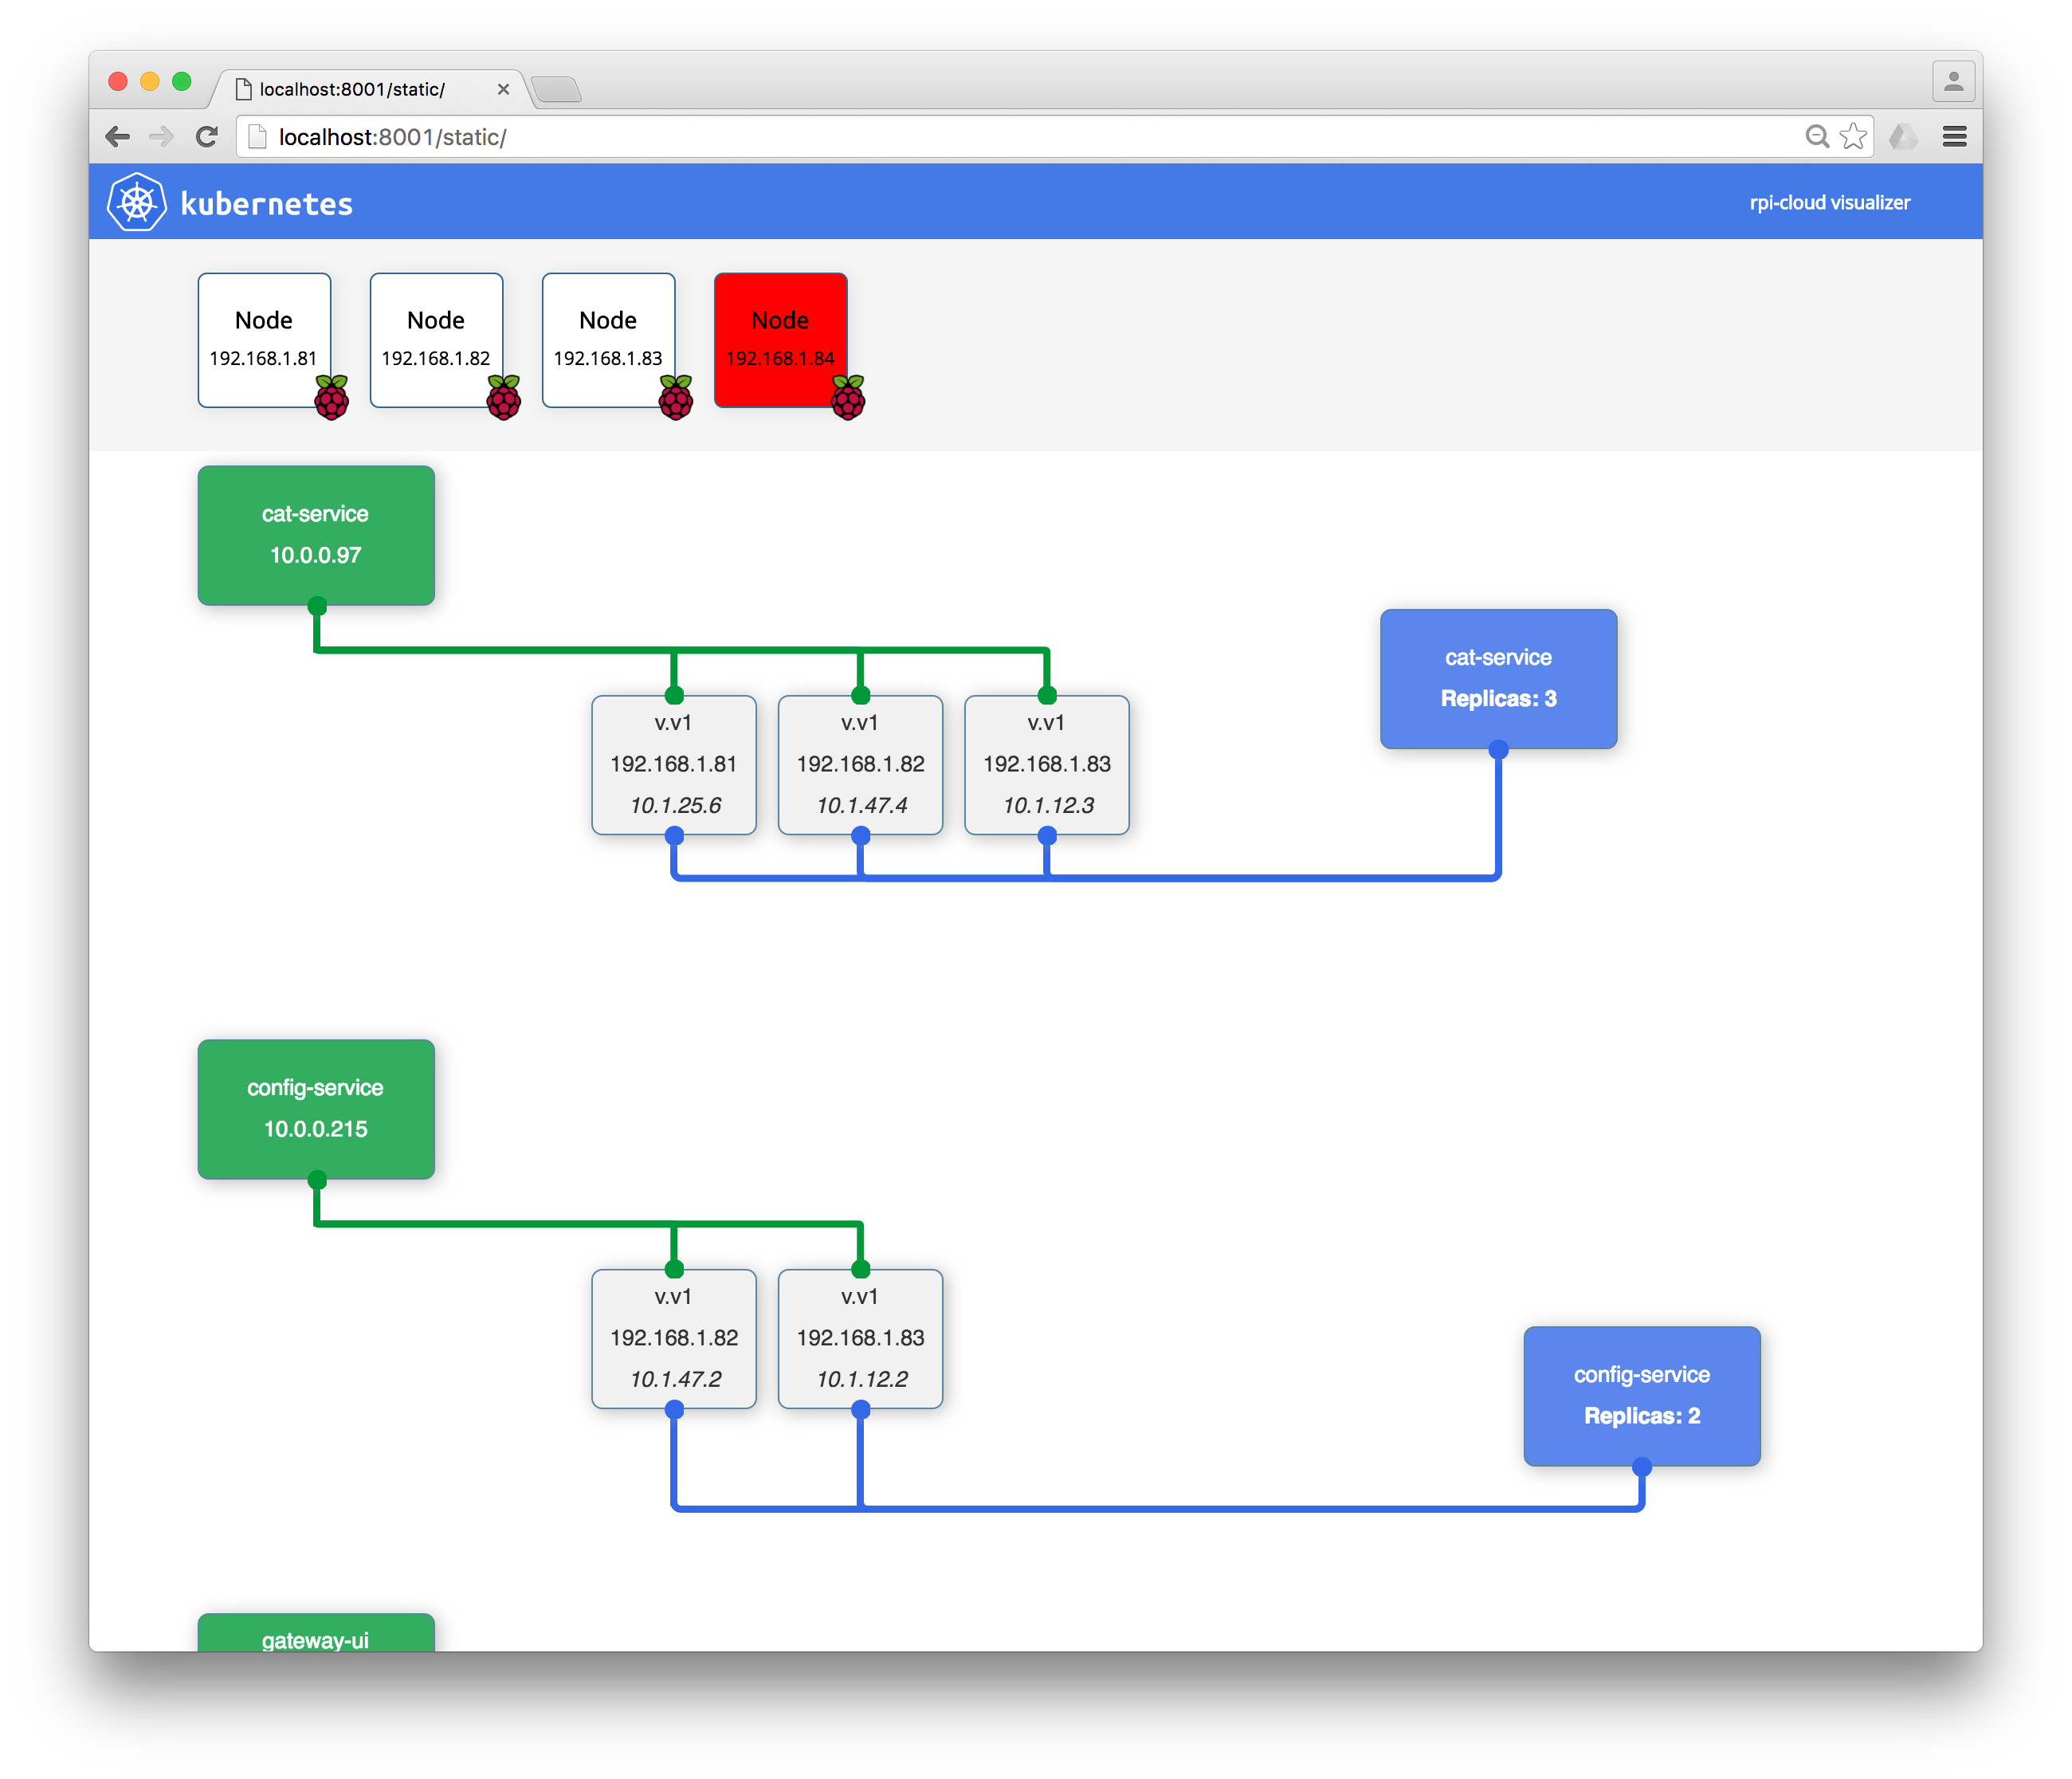
\includegraphics[width=7cm]{figures/visualizer/node_fail_recovered} }}%
    \caption{Visualization of Node Failure}%
    \label{fig:visualizer_node_failure}%
\end{figure}

\noindent 
The top row indicates the status of each node, and the red color indicates that the last node is not responding. Each green box corresponds to a running \textit{service}. The services are connected to \textit{pods} of varying colors. The pod color indicates whether a pod is running, pending or terminating. The pods are controlled by \textit{deployments} that are shown as blue boxes. \\
As seen in Figure~\ref{fig:visualizer_node_failure}, the overview of the cluster changes dynamically when the state of the cluster is changed. Figure~\ref{fig:visualizer_node_failure}(a) shows that one of the nodes is not reporting heartbeats to the API server. (b) shows Kubernetes rescheduling the pod running on the failing node to maintain the desired state of the deployment. (c) shows the recovery to the desired state. Lastly (d) everything is cleaned up and fully recovered.

\noindent
Brendan Burns, co-founder of the Kubernetes project, has created the original visualization tool. This tool has been open sourced and a lot of contributions have been made by, among others, Ray Tsang (saturnism) and Arjen Wassink (awassink). We have forked their repository and made some additions. The additions to the visualizer made during this master's thesis are, among others, fixing a memory leak in the original code. Drawing of nodes in the DOM kept being overlayed every 3 seconds. The result of having the visualizer open for longer periods made it heavy to interact with. Furthermore, the upgrade from Kubernetes 1.1 to 1.2 resulted in issues. ReplicationController were substituted with replica sets and deployments. We updated the visualizer to work with 1.2.
%!TEX root = ../../master.tex

\subsection*{Application Layer}
The two previous sections described how Kubernetes runs and manages containerized applications (Figure~\ref{fig:flow_spring_software}). Now we will focus on the applications running on top of the infrastructure.
The application layer is not limited to a single language or framework since Docker containers are used. In order to experiment with microservices, a microservice chassis framework is chosen: Spring Boot and Spring Cloud. These frameworks make it easy to get up and running with a microservice architecture in Java. Furthermore, Spring Boot and Spring Cloud offer many relevant cloud computing libraries that easily can be included in projects. Multiple Netflix Open Source libraries are accessible through Spring Cloud e.g. an implementation of a circuit breaker for synchronous communication (Hystrix) and an implementation of the API Gateway pattern (Zuul). These libraries and examples of implementing them are described in further details in Appendix~\ref{appendix:application_layer}. \\


\noindent
KubeCloud is used as a presentation item as well as a practice item. In order to accommodate the role as a presentation item a demo project demonstrating some concepts of microservices, Docker and Kubernetes has been implemented. Secondly, the demo project supports the role as a practice item by providing a reference point for the students to get started. The demo project is a simplified microservice architecture to keep the initial complexity and understanding of the system low. The architecture contains four services as depicted in Figure~\ref{fig:demo}.

\begin{figure}[H]
    \centering
    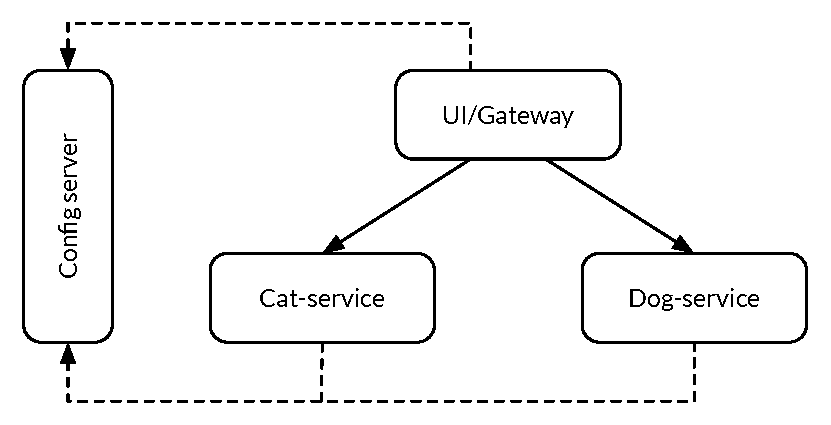
\includegraphics[width=9cm]{figures/demo_architecture}
    \caption{Architecture of Demo Application}
    \label{fig:demo}
\end{figure}

\noindent The four services are:
\begin{itemize}
  \item \textbf{Config-server}: The config server is implemented with the Spring Cloud Config, and acts as a central configuration management hub.
  \item \textbf{UI/Gateway}: The UI/Gateway is an implementation of the API Gateway pattern along with the graphical user interface (GUI) of the application.  
  \item \textbf{Cat-service}: The cat-service is a RESTful service, returning a list of cat-objects 
  \item \textbf{Dog-service}: The dog-service is a RESTful service, returning a list of dog-objects.
\end{itemize}

\noindent 
The graphical user interface makes requests to the API Gateway that then directs the calls to the specific service. The application is shown in Figure~\ref{fig:example} in which the data from cat-service is shown in Figure~\ref{fig:example}(b).

\begin{figure}[H]%
    \centering
    \subfloat[UI Gateway]{{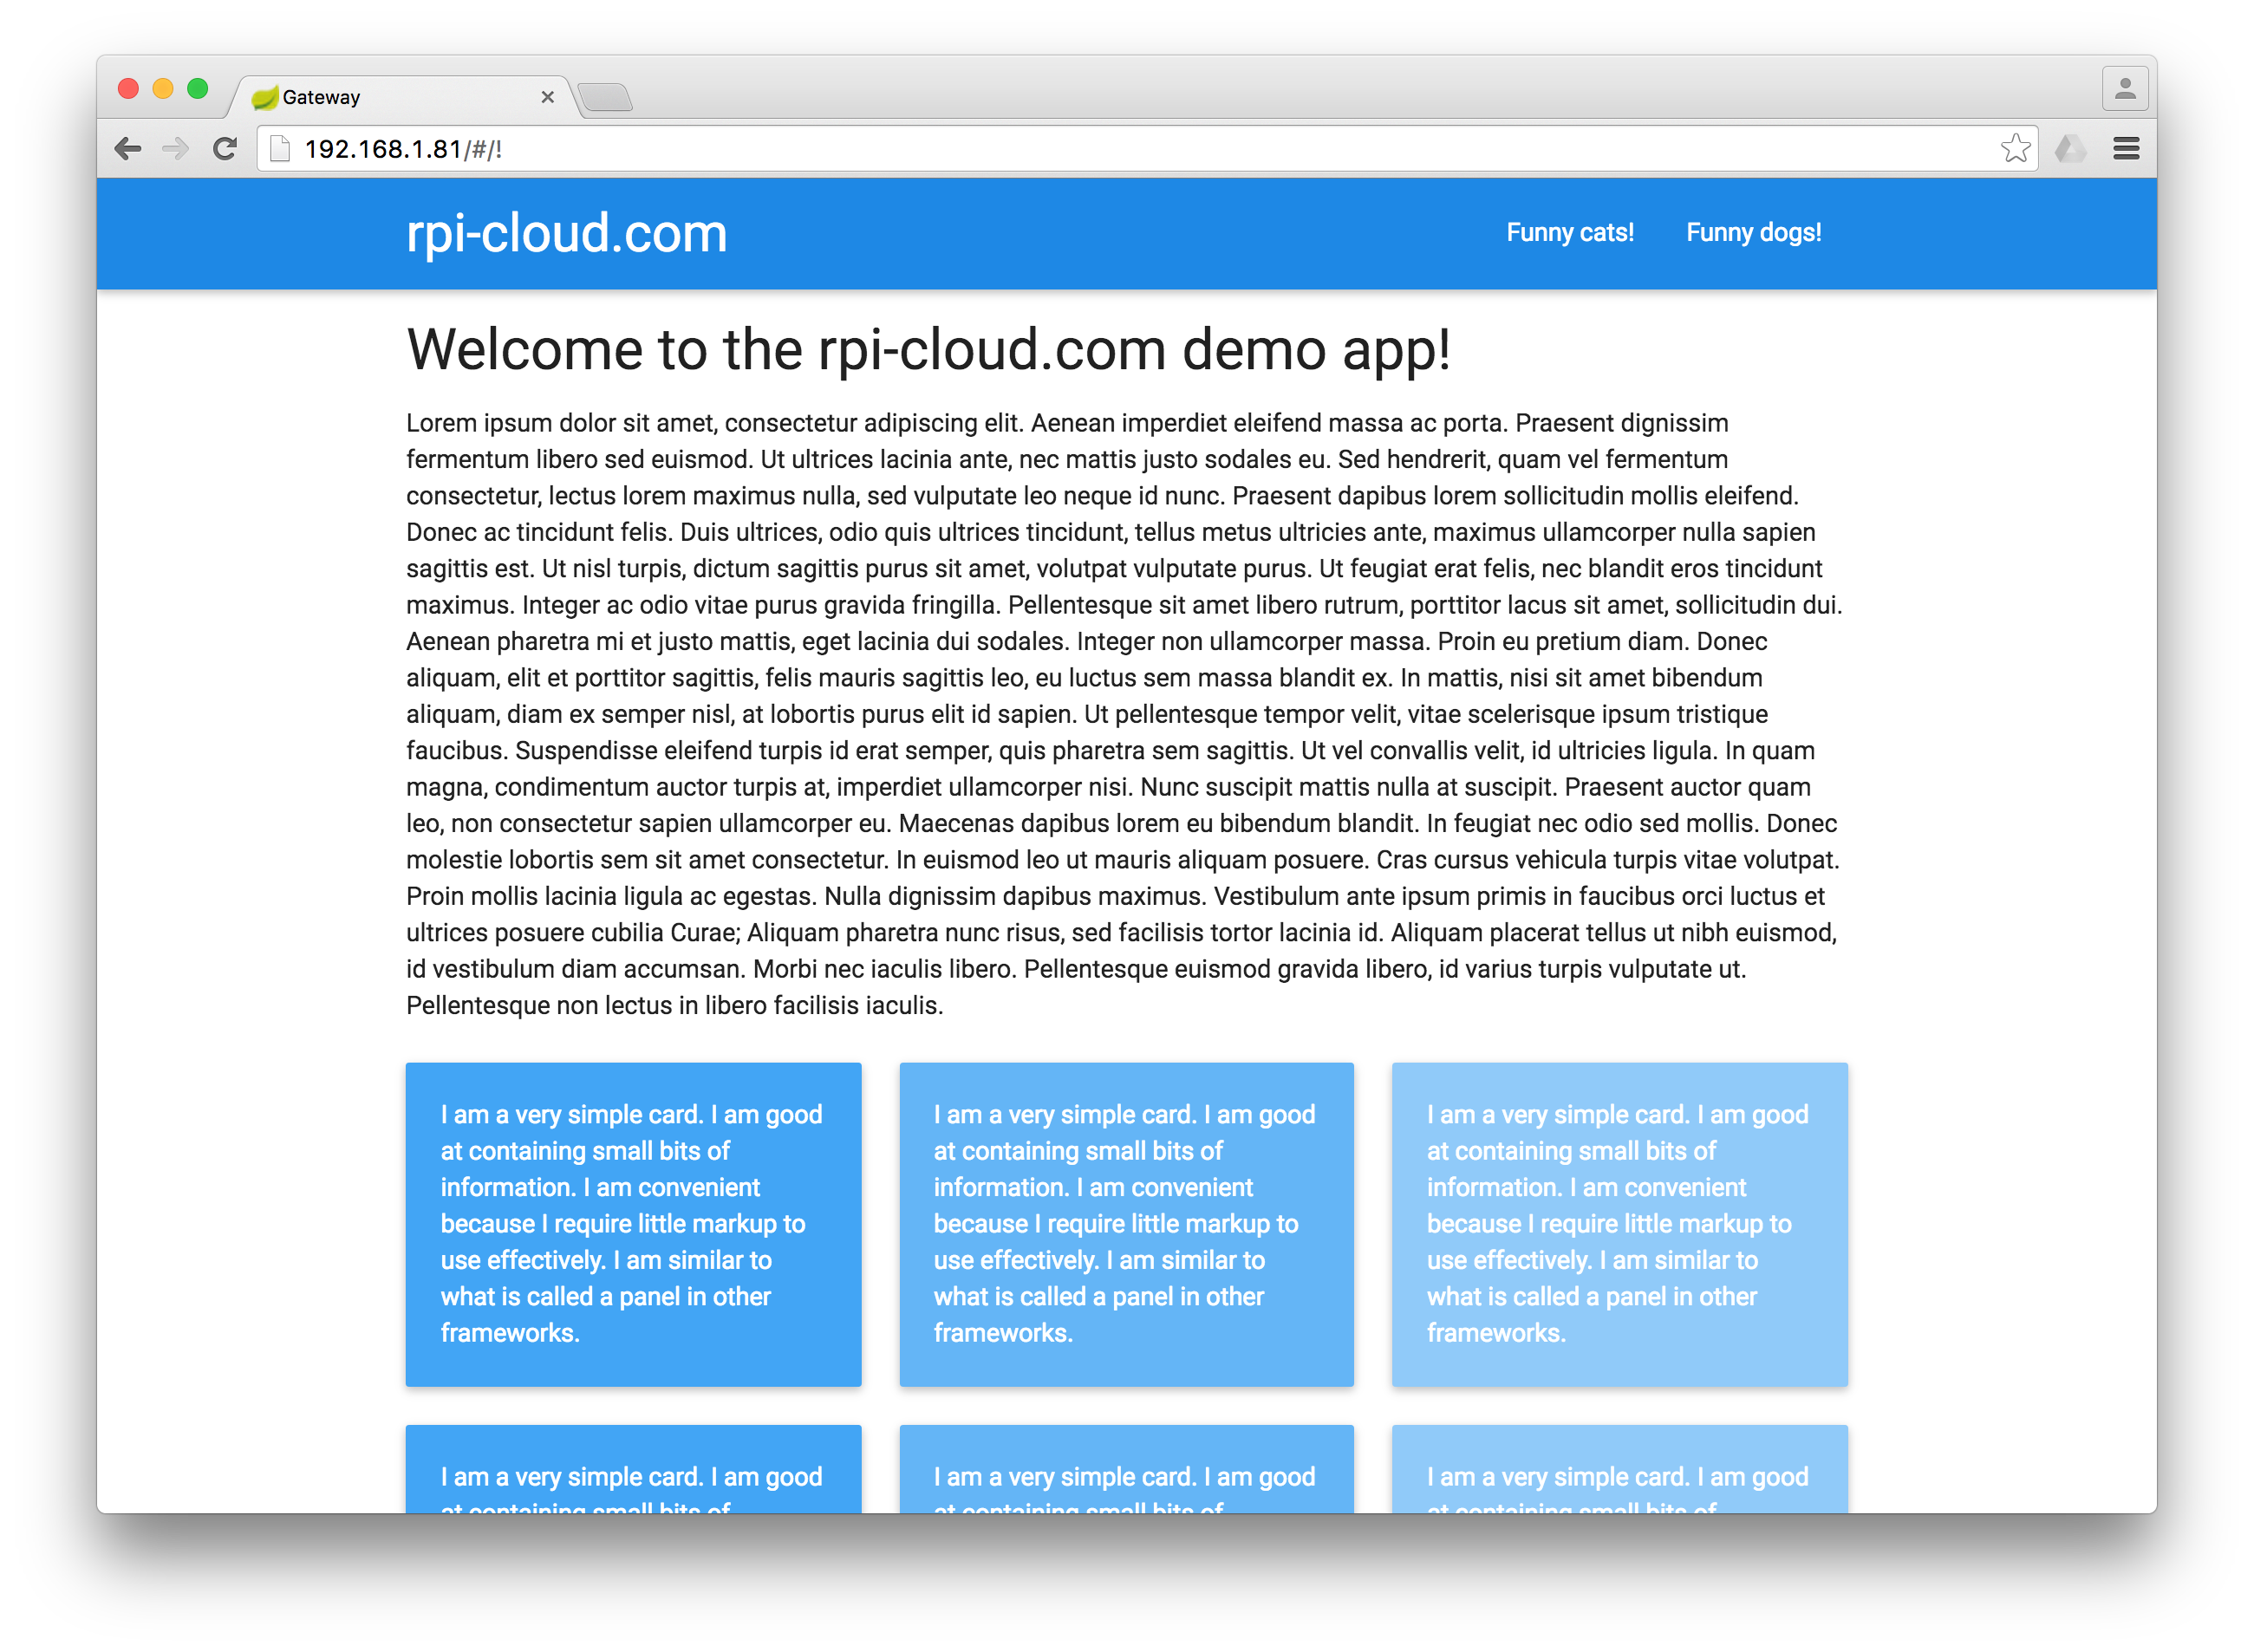
\includegraphics[width=7cm]{figures/demo/home} }}%
    \qquad
    \subfloat[Cats v2]{{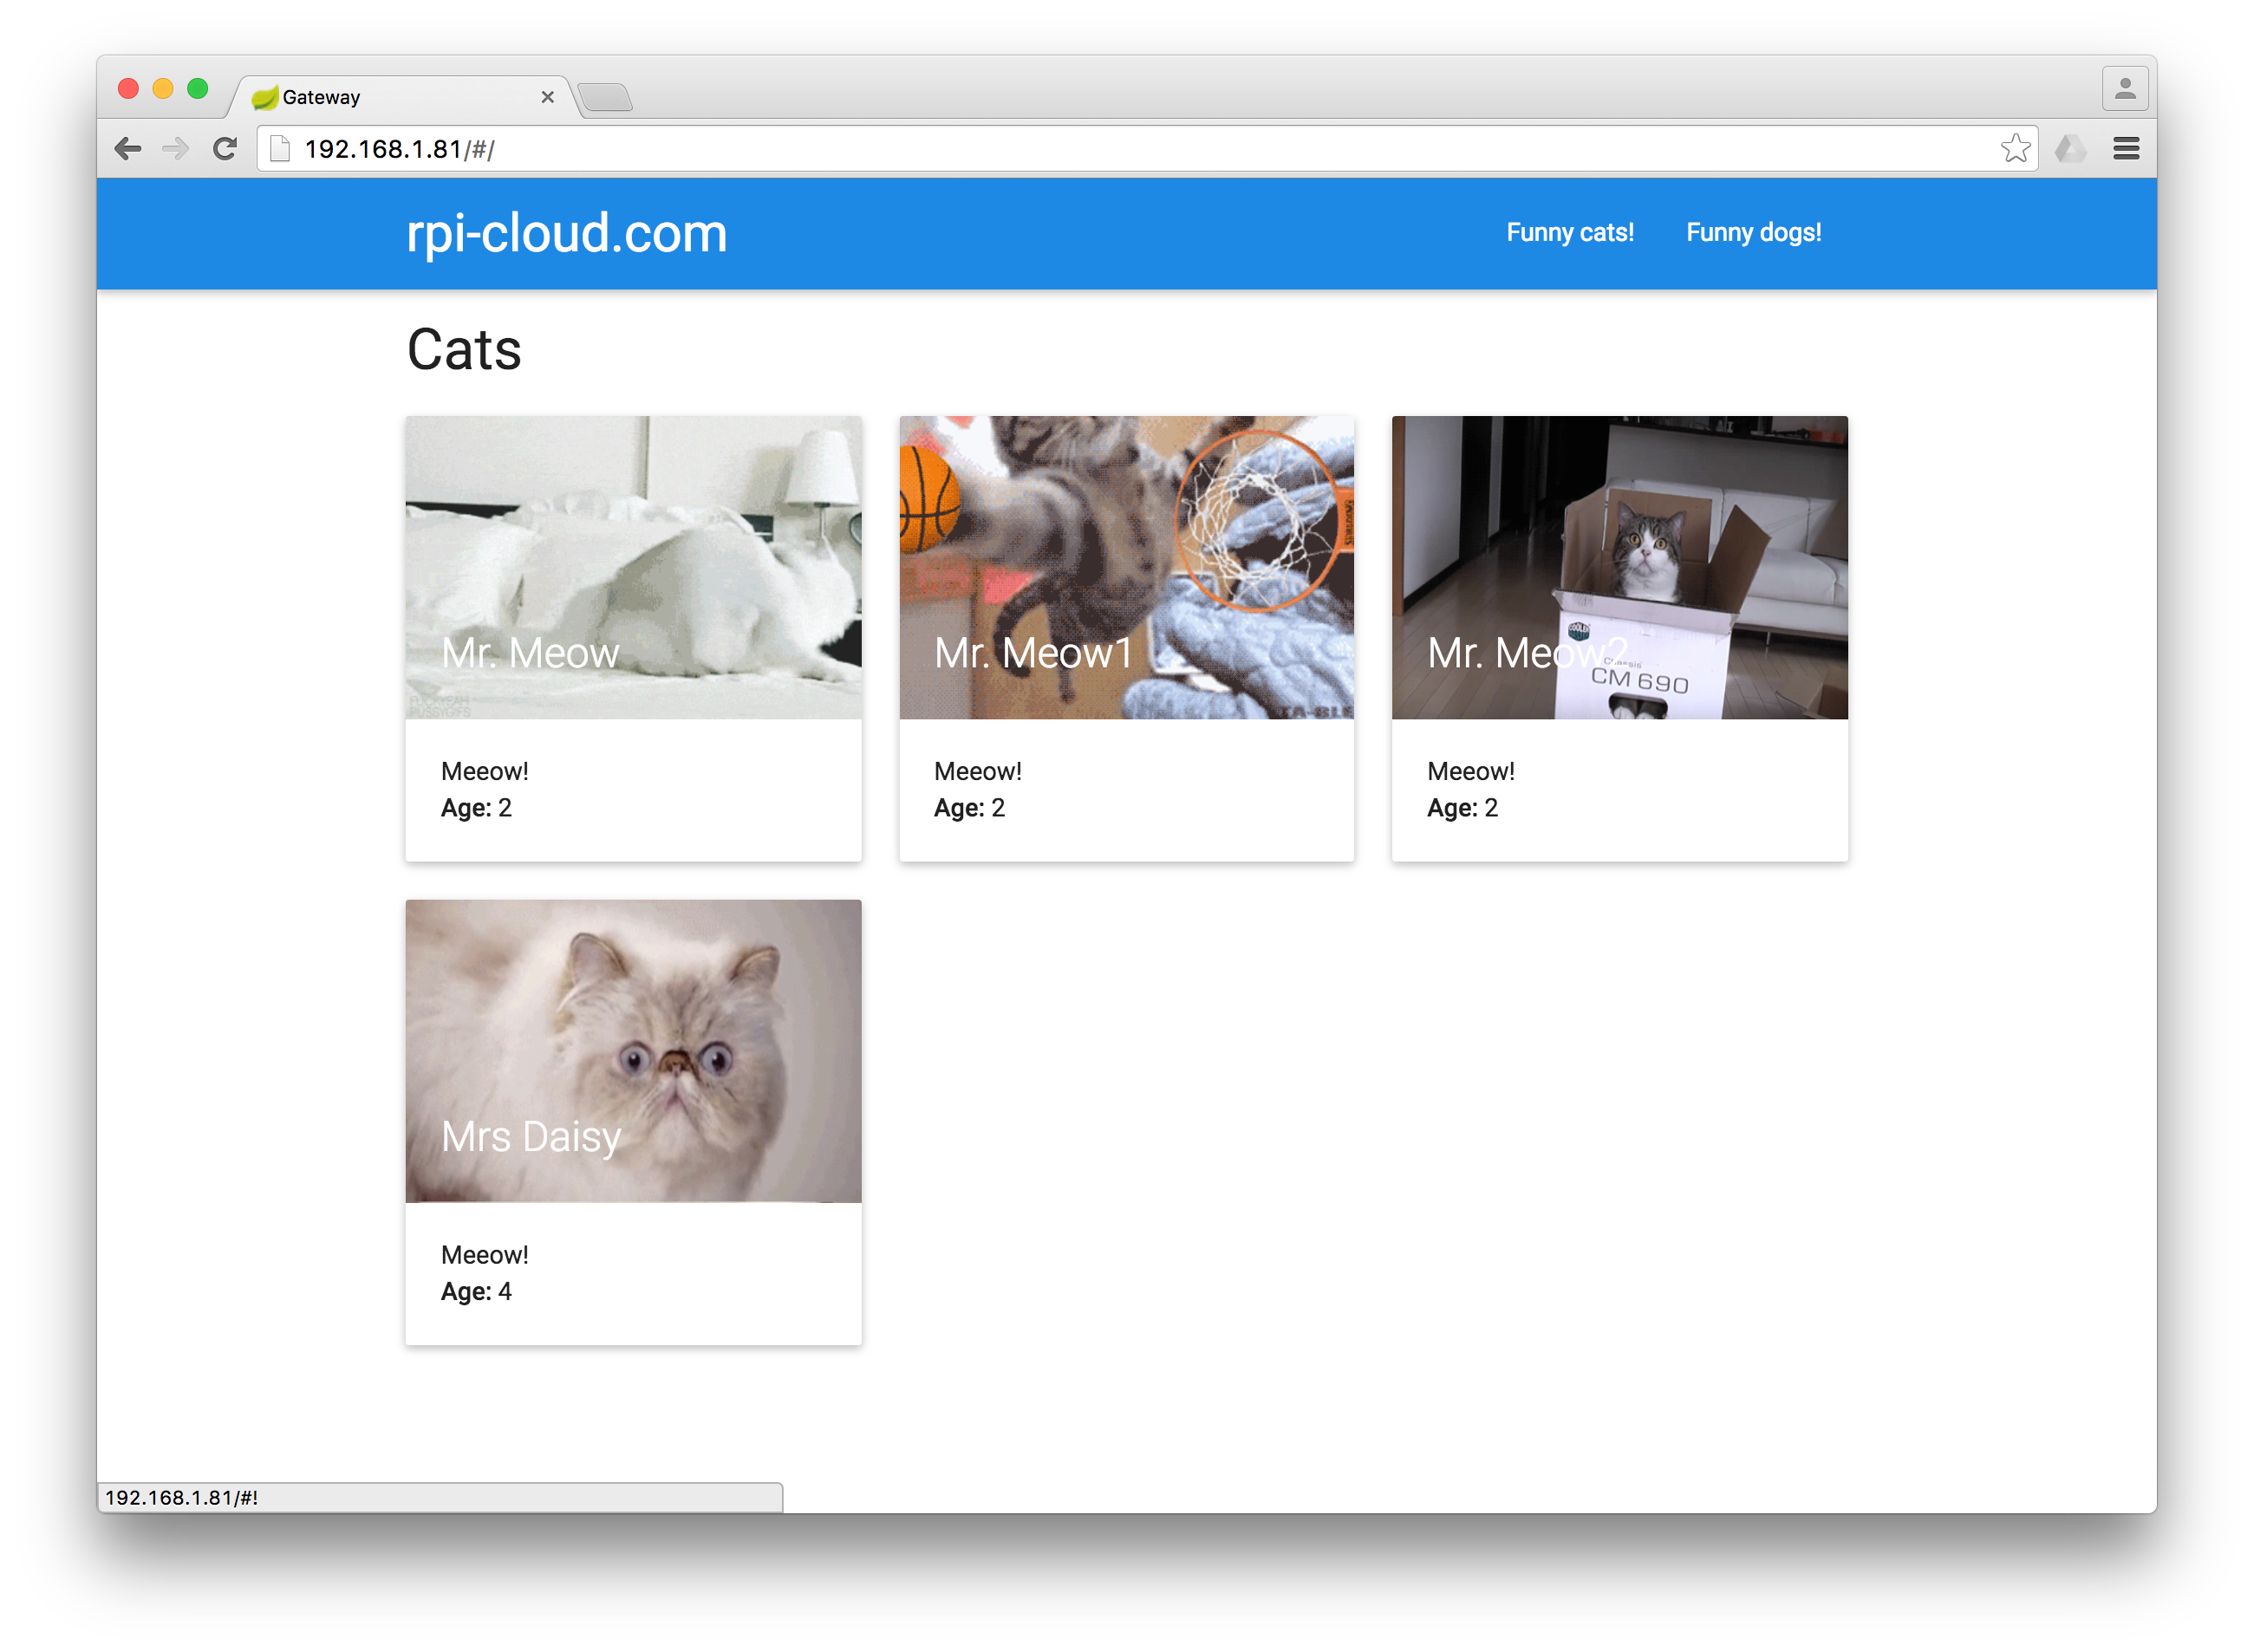
\includegraphics[width=7cm]{figures/demo/cats_v2} }}%
    \caption{Screenshots of Demo Application}%
    \label{fig:example}%
\end{figure}

\noindent
The previously mentioned DNS add-on for Kubernetes is used for service discovery for the individual microservices in this dynamic environment. The DNS add-on allows inter-service communication by using the Kubernetes services' names instead of IPs. Figure~\ref{fig:dns} shows an example where a service makes a request to \textbf{http://config-service}. This service name will then be attempted resolved on the host by looking up the designated DNS services. The resolv.conf file, from the host machine, contains the IPs of the DNS services. The KubeDNS virtual IP is added to resolv.conf by kubernetes-on-arm. KubeDNS is then contacted and looks up \textbf{config-service} in etcd. If found, the resolved IP will be sent back, and the service name is resolved to a virtual IP that the request is sent to as specified in Figure~\ref{fig:flannel}. 

\begin{figure}[H]
    \centering
    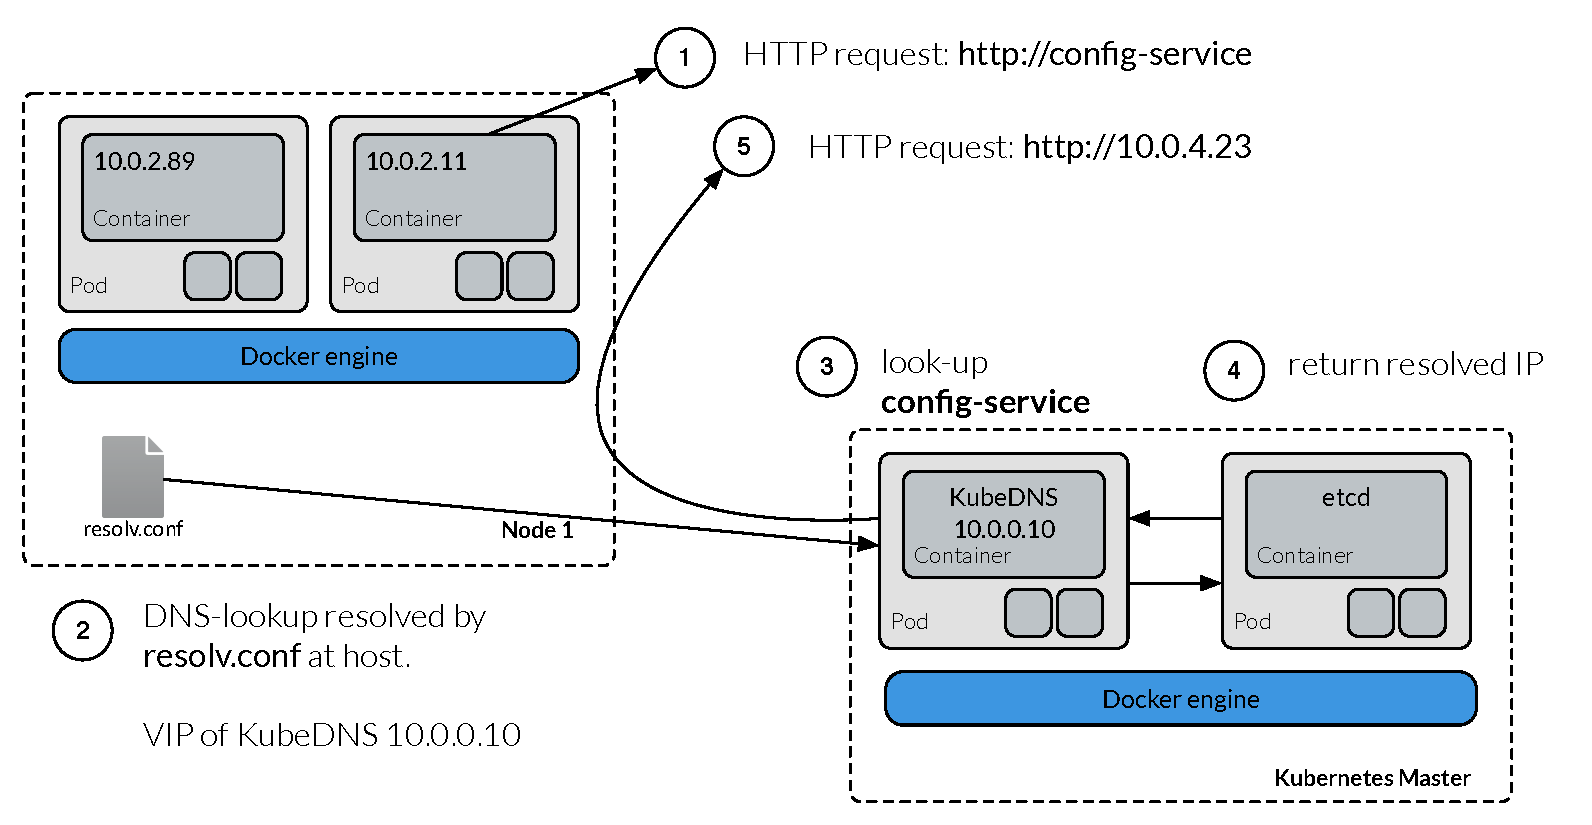
\includegraphics[width=12cm]{figures/kubernetes/kubedns}
    \caption{KubeDNS}
    \label{fig:dns}
\end{figure}
%%!TEX root = ../../master.tex

\section{Stability}
Making the Raspberry Pi Kubernetes cluster stable
Transportation
%!TEX root = ../../master.tex

\section{Load and Stress Testing}
When applications are developed and deployed in KubeCloud, we need to simulate user traffic on the cluster to apply real use cases. KubeCloud then becomes a controlled test environment for cloud computing research. In order to simulate traffic and experiment with how applications respond to different traffic loads, different attacks can be made. There are two different ways of attacking the application: \textit{load} and \textit{stress testing}. A load test is \textit{"a test focused on determining or validating performance characteristics of the software under test when subjected to workload models and load volumes anticipated during production operations"} \cite{techtarget2016testing}. In a stress test the subject to workload is pushed beyond the anticipated production operations.
\noindent Both types of tests have been performed in this thesis. In order to perform load and stress testing Vegata\footnote{\url{https://github.com/tsenart/vegeta}} and Gatling.io\footnote{\url{http://gatling.io/}} have been used. Vegeta allows for a constant request rate against a target whereas Gatling records usage scenarios and replay them.
%!TEX root = ../../master.tex

\section{Benefits and Limitations}
The benefits and limitations met in the process of designing and implementing KubeCloud will be described in this section.

\subsection*{Benefits}
\textbf{Hands-on} \\
The cluster allows students to interact and experiment with a physical model of the concepts. Raspberry Pis are used as server machines (Kubernetes nodes) instead of spinning up virtual machines on a cloud provider. This enables the students to inject failures such as pulling the network cable, attacking with a large traffic load, etc. \\

\noindent \textbf{Visualization} \\
The visualization tool is not restricted to Kubernetes in a Raspberry Pi cluster. The representation of the nodes makes it easier to understand where workloads are scheduled and how the cluster maintains the desired state. \\

\noindent \textbf{Affordable Test Environment} \\
Buying a test environment is expensive in terms of hardware, cooling, installation and power consumption. An example from the University of Helsinki spending around one million Euros without cooling systems \cite[p. 170-171]{abrahamsson2013bolzano} illustrates how expensive this solution is. By contrast, KubeCloud is cheap, portable, and has low power consumption. KubeCloud is not as performant as a full-size data center, but the same concepts and network errors can be experimented with in a closed test environment. \\

\noindent \textbf{Transportable} \\
The fact that KubeCloud is transportable allows students to use the cluster whenever they want to. No expensive installation of a large data center is necessary. \\

\noindent \textbf{Configurable} \\
Since KubeCloud can be configured in numerous ways, the clusters can also be used with a varying amount of workers per master. The physical design allows the physical clusters to be assembled with a varying amount of Raspberry Pis. \\

\noindent \textbf{Flexible} \\
Another benefit is KubeCloud's flexibility in terms of what software it can run. Docker allows everything that can be packaged into a Docker image (on ARM) to run in the cluster. This makes it easy to have different runtimes available without causing conflicts between different versions among the users. Since Docker can be used without Kubernetes it is not needed to understand Kubernetes to use the cluster. 

\subsection*{Limitations}
\textbf{ARM Architecture} \\
The largest limitation is that Raspberry Pis use the ARM architecture. The benefit of low price and lower power consumption comes with trade-offs. Most developer machines do not use ARM architecture which leads to an unfortunate situation concerning Docker. Containers must be built on an ARM machine or cross-compiled, but this introduces the issue of different execution environments that Docker is trying to solve in the first place. Running ARM-built containers, on the other hand, might be accessible from a developer machine in the near future\footnote{\url{http://blog.hypriot.com/post/first-touch-down-with-docker-for-mac/}}. The fragmentation that ARM architecture introduces is, though, still unfortunate in regards to what images can be applied. \\

\noindent \textbf{Build/Deployment Process Slow} \\
When a microservice is updated with new functionality, it takes some time before it is running in the cluster. In the process a new Docker image must be built and pushed to a registry, configuration files updated, and a deployment with the new image started. Because of the Raspberry Pi's performance pulling and pushing Docker images take some time. This manual process could be automated by leveraging concepts from continuous delivery. \\

\noindent \textbf{Power Supply} \\
In KubeCloud, each Raspberry Pi has its own power supply connected to a power strip. This results in many cables, and a better solution would have been a power hub built into the physical construction. However, due to budget constraints, this was not possible. \\

\noindent \textbf{Stability Concerns} \\
In order to sustain a stable Raspberry Pi cluster, all nodes must be shut down correctly. The portability of the cluster introduces a risk of stability issues opposite a datacenter in a basement. Pulling the power plug can lead to corrupt SD cards or invalid state in the Kubernetes cluster. 


















% INTRO FROM OLD EXPERIMENT

%\textbf{Argumentér for valg af Raspberry Pi}
%
%\section{Elements of RPi cloud stack}
%Hvordan kan man gøre cloud håndgribelig. Hvilke muligheder har vi? Præsentér muligheder.
%
%\section{Designing a RPi cluster}
%Argumentér for valg af dele i stakken.
%
%\section{Stability (issues)}
%Open source, hobby, vores bidrag i forhold til stabilitet. \\
%Matching Kubernetes, Docker, and OS versions
%
%%!TEX root = ../../master.tex





% This section will describe the experiments conducted throughout this present master thesis. These experiments are divided into two main categories, that are still highly cohesive. The two categories are the experiments regarding the learning experience and the Raspberry Pi cluster as a learning object. Lastly the experiments concerning resilience in relation to finding ways that will highlight the problems and solutions to distributed computing. The experiments concerning resilience will focus upon the anti-patterns and patterns described by Michael Nygard and the resilience that Kubernetes as a platform will provide. These experiments and their results should provide the basis of determining if the taken approach will help aligning the students mental model with the real world of cloud computing and distributed systems.
